\chapter{EpiNeRF: epipolar-based feature attention for single-image novel view synthesis}
\label{chapter:epinerf}

\chapterwithfigures{\nameref*{chapter:epinerf}}
\chapterwithtables{\nameref*{chapter:epinerf}}

\ifthenelse{\boolean{skipEpiNeRF}}{\endinput}{}

Over the past few years, significant advancements have been made in \ac{NVS} from a single image using \ac{NeRF}. Traditional approaches typically involve \ac{NeRF}'s input conditionning with spatial image features, that are aligned to each source pixel and generated by an encoder-decoder \ac{CNN}. However, we believe that integrating target-aligned features can improve the network's abilities to handle occlusions and unseen viewpoints in single-image \ac{NVS}. We introduce EpiNeRF, a multi-stage training architecture designed to leverage target-aligned features. The first stage involves learning target-aligned features from source-view features through a feature-\ac{NeRF}, called NeRFeature, using a teacher-student distillation method. Source and target aligned features are then combined in an epipolar attention module, which balances and correct how 3D points should be sampled along a ray during training. Our extensive experiments on both synthetic and real-world datasets emphasize the importance of target-aligned features, which are usually unavailable in single-image \ac{NVS} frameworks.

\section{Introduction}
% [1st paragraph] - Why is the problem important. 
\ac{NVS} is a crucial computer vision problem due to its wide range of applications in fields such as \ac{VR},\ac{AR} or 3D reconstruction. Few-shot \ac{NVS} aims to generate images from unobserved viewpoints using only a limited number of source images and their corresponding camera pose information.

% [2nd paragraph] - Why is the problem difficult. 
Single-image \ac{NVS} is inherently ill-posed, as a single view may not provide sufficient visual information to generate a novel viewpoint. Handling unforeseen elements as well as occlusions becomes particularly hard in this context. Leveraging 3D priors \citep{saito2019pifu,johari2022geonerf} is essential for addressing these challenges, as it enables deep architectures to gain a fundamental understanding of the underlying 3D scene structure.

% [2bis] - Limitation and motivation for our work. 
Recent works \citep{yu2021pixelnerf,li2022symmnerf,lin2023vision} leveraging generalizable NeRF in single-image \ac{NVS} extensively rely on the source view to produce a low-resolution 2D feature $\textbf{F}_{s}$ volume that conditions the radiance field. Such a volume is bilinearly interpolated to get \textit{local} pixel-wise feature, aligned with the input image. When source and target views are far from each others, occlusions and unobserved parts in the source domain lead to misaligned and coarsely-local feature on $\textbf{F}_{s}$, producing a non-optimal conditioning. 

% [3rd paragraph] - What is your key idea ? You can point to the teaser figure. 
Our work therefore tries to address such a limitation in two main stages. First by producing target-aligned features from a feature radiance field, learn by distilling pre-trained 2D \ac{CNN} features into a 3D \ac{NeRF}. These target-oriented features are then involved (with their source-aligned counterparts) in a light epipolar attention-based mechanism. The weights sampling distribution that took place in the volume rendering procedure is shrunk around regions where source and target features match, allowing a better spatial 3D points sampling.

% [4th paragraph] - Give the important technical details
As depicted in Figure \ref{fig:overview}, the training of our complete EpiNeRF architecture \textit{(bottom part)} involves two main stages.  First, the feature radiance field, called NeRFeature, is trained through a feature distillation process \textit{(top-left)}. Then, the light epipolar attention-based module \textit{(top-right)} is introduced. These two preliminary steps allows EpiNeRF to finally be fine-tuned with the epipolar attention module, which uses the target-aligned features from NeRFeature to refine the volume rendering equation and emphasize on 3D points where source and target features align.
 
% [5th paragraph] -How do you evaluate your method ? What are the most impressive results ?
We evaluate EpiNeRF against several state-of-the-art methods on both synthetic (ShapeNet-SRN \citep{sitzmann2019scene}) and real-world (Standford Cars \citep{krause20133d}) datasets. In contrast to previous methods that rely solely on those source-view features, our feature epipolar attention module effectively accounts for occlusions through its target-aligned feature considerations. 

% [6th paragraph] - A summary of your contribution
Our contributions are threefold and can be summarised as follows: 
\begin{enumerate}
   \item A  feature radiance field, called NeRFeature. Given an input source-aligned feature with a camera transformation, NeRFeature infers the corresponding target-aligned deep feature. The light feature distillation procedure involved to train NeRFeature do not require any heavy foundation models (Section \ref{subsec:nerfeature}). 
    \item A simple yet effective epipolar-based attention mechanism that relies on these source and target-aligned features. It dynamically corrects the weights sampling distribution during volume rendering (Section \ref{subsec:epipolar_att}). 
    \item A novel generalizable NeRF architecture for single-image \ac{NVS} that we termed EpiNeRF. It directly leverages both the NeRFeature radiance field and our epipolar attention module to reweight the volume rendering equation in regions where source and target features align most closely (Section \ref{subsec:epinerf}).  
    
\end{enumerate}


\section{Related work}

\noindent\textbf{Single-image novel view synthesis.} Novel view synthesis aims to generate an image of a scene from a an unobserved viewpoint using a set of posed images, i.e. images with their associated camera poses. Early approaches in the literature rely on fully convolutional-based networks ~\citep{kim2020novel,hou2021novel,guo2022fast,landreau2022epipolarnvs}. Emergence in 2020 of NeRF ~\citep{mildenhall2020nerf} based models have significantly influenced the way single-view \ac{NVS} architectures ~\citep{yu2021pixelnerf,li2022symmnerf,lin2023vision} are now built. These architectures all consider an image encoder to condition the radiance field. Whereas the latest research in single-image \ac{NVS} push toward heavy image-conditioned diffusion models ~\citep{chen2023single,gu2023nerfdiff,chan2023genvs}, recent advances in foundational 3D reconstruction models makes it possible to capture an object's full 3D structure from just one view ~\citep{liu2023zero,zou2023triplane}. However, these diffusion-based architectures remain complex to train and have poor speed inference performances.  

\noindent\textbf{Generalizable NeRF conditioning.} In its original formulation, a set of posed images is sufficient to design and train a \ac{NeRF} architecture on a single static scene.

However, above formulation prevents \ac{NeRF} networks to generalize across multiple scenes. Many recent works use deep feature volumes to condition their neural architecture ~\citep{wang2021ibrnet,chen2023matchnerf} in few-shots \ac{NVS}. PixelNeRF ~\citep{yu2021pixelnerf} is one of the first works to address these limitations in single-image \ac{NVS} by locally conditioning its radiance field with pixel-wise, source-aligned features from a \ac{CNN} encoder-decoder. This \textit{local}, input based conditioning is now widely adopted in the devoted literature \citep{jang2021codenerf,li2022symmnerf,lin2023vision}.

\noindent\textbf{Feature distillation in NeRF.} A radiance field can be extended to output features beyond the RGB space, as long as a corresponding supervisory signal exists for the training phase. Work from \citep{hinton2015distilling} lay the ground for feature distillation by focusing on knowledge transfer and model compression issues. Few other methods already distill feature from 2D models (such as \ac{CNNs} or {ViT} \citep{dosovitskiy2020vit}) into 3D using neural radiance fields \citep{kobayashi2022decomposing}. While \citep{ye2023featurenerf} learn a radiance field  by distilling feature from a 2D foundation model \citep{oquab2023dinov2}, we propose a lighter feature distillation procedure. 

\section{Background: Neural Radiance Fields}


\ac{NeRF} have emerged as a revolutionary technique to reconstruct 3D static scenes and render novel views. Introduced in 2020 \citep{mildenhall2020nerf}, such a neural field leverages \ac{MLP} to generate high-fidelity images of a scene from a sparse set of input images. \ac{NeRF} captures both geometry and lighting in a 3D environment, providing a powerful framework for synthesizing views from arbitrary perspectives.

\subsection{General overview}

Given a 3D point in world space $\mathbf{X} \in \mathbb{R}^{3}$ along a ray and its viewing direction $\mathbf{d} \in \mathbb{R}^{3}$, a vanilla RGB \ac{NeRF} is defined through a density $\sigma(\mathbf{X})\in \mathbb{R}_{+}$  and a RGB colour $c(\mathbf{X},\mathbf{d}) \in \mathbb{R}^{3}$. A radiance field models a scene as a continuous function $F_{\theta}$ that predicts both the color and density of points in 3D space: 

\begin{equation}
  F_{\theta}(\mathbf{X},\mathbf{d}) = c,\sigma
\end{equation}

The volumetric density $\sigma$ corresponds to the amount of light absorbed or scattered as a ray passes through $\mathbf{X}$. Both color and density are obtained from $F_{\theta}$ network, which is usually a shallow \ac{MLP}.

To synthesize images from novel viewpoints, \ac{NeRF} employs a differentiable volume rendering operation \citep{max1995optical}, which involves integrating the colors and densities along rays cast through the scene. In its continuous form, a ray originating from a camera at position \(\mathbf{o}\) and passing through a pixel on the image plane is defined through $\mathbf{r} = \textbf{o} + t\times \mathbf{d}$. The rendered RGB color $\hat{c}$ along the ray is then given by: 

\begin{equation}
  \label{eq:vr-nerf}
  \hat{c}(\mathbf{r}) = \int_{t_n}^{t_f} T(t) \cdot \sigma(\mathbf{r}(t)) \cdot c(\mathbf{r}(t),\mathbf{d}) dt
\end{equation}

with: 

\begin{equation}
  T(t) = 1 - e^{-\int_{t_n}^{t}\sigma(\mathbf{r}(s)ds)}
\end{equation}

the accumulated transmittance, which accounts for the attenuation of light due to the medium, along the ray $\mathbf{r}$.  The pair $[t_{n},t_{f}]$ defines the near and far bound of the ray. This volume rendering equation means that color observed at a specific pixel location is a weighted summation of the contributions from all the points along the ray. The density $\sigma$ somehow simulates the physical properties of light as it travels through the scene. Higher density values indicate more opaque materials that scatter light, while lower values correspond to transparent materials.  

To render a view from such a radiance field, one need to estimate $\hat{c}(\mathbf{r})$ for each camera ray traced through the pixels of the target camera. 

\subsection{Discretized formulation}

Such an integral defined in Equation \eqref{eq:vr-nerf} has to numerically be approximated through quadrature. A stratified sampling approach has thus been implemented in the seminal \ac{NeRF} paper \citep{mildenhall2020nerf} to split the interval $[t_{n},t_{f}]$ into $N_c$ evenly-spaced bins, where $N_c$ points, termed $\mathbf{X}^{(i)}$, are uniformly sampled within each interval: 

\begin{equation}
  \mathbf{X}^{(i)} \sim \mathcal{U}\left[ t_{n} + \frac{i-1}{N_c}(t_{f} - t_{n}),t_{n} + \frac{i}{N_c}(t_{f} - t_{n}) \right]
\end{equation}

The composite RGB color $\hat{c}$ along the ray is thus discretized and computed through: 
\begin{equation}
\label{eq:main_nerf}
\hat{c}(\mathbf{r})  = \sum_{i=1}^{N_c}T^{(i)}\alpha^{(i)}c(\mathbf{X}^{(i)},\mathbf{d}) = \sum_{i} \omega^{(i)}c(\mathbf{X}^{(i)},\mathbf{d})
\end{equation}

with: 
\begin{equation}
\alpha^{(i)} = (1-\exp^{-\sigma(\mathbf{X}^{(i)})\delta_{i}})
\end{equation}
The term $\delta_{i} = \mathbf{X}^{(i+1)} - \mathbf{X}^{(i)} $ refers to the distance between two consecutive samples along the ray.

The field $\alpha$ should be interpreted as the probability of hitting a particle over an infinitesimal distance $\delta_{i}$ traveled along the ray $\mathbf{r}$. The term $1 - \alpha^{(i)}$ thus represents the probability of not encountering any particles over such a displacement. Finally, the transmittance $T^{(i)} = \prod_{j=1}^{i-1}(1-\alpha^{(j)})$ is the probability of not hitting any particles over the interval $[t_{n}, \mathbf{X}^{(i)})$ while traveling along $\mathbf{r}$. It can also be easily refactored through: 
\begin{equation}
T^{(i)} = \exp\left( - \sum_{j=1}^{i-1}\sigma(\mathbf{X}^{j})\delta_{j}\right)
\end{equation}

The final weight term: 
\begin{equation}
\label{eq:weights}
    \omega^{(i)} = \alpha^{(i)}T^{(i)} = \alpha^{(i)}\prod_{j=1}^{i-1}(1-\alpha^{(j)})
\end{equation}
in the final composite RGB color $\hat{c}$ is therefore interpreted as the likelihood that the ray terminates exactly at index $i$. 

\subsection{Hierarchical volume sampling}

\ac{NeRF}'s authors found in their original experiments that stratified sampling was unsufficient to densely sample the 3D scene. Indeed, solely quering $N_{c}$ points along ray might leave regions unexplored or occluted. Increasing the number of bins might appear inefficient from a computational perspective since too many points could be sampled and queried on empty areas. The hierarchical volume sampling strategy tries to tackle such a drawback by re-distributing sampled points along rays in proportion to their anticipated impact on the final rendering. 

The piece-wise constant probability density function obtained from the normalized weights $\omega^{(i)}/ \sum_{j=1}^{N_c}\omega^{(j)}$ distribution is threfore used to sample a second set of $N_f$ points, using inverse transform sampling.

The original \ac{NeRF} paper therefore implements not just one radiance field but two: a coarse one, which is queried on the $N_c$ points from the stratified sampling, and a second finer one, which is called upon the $N_{c}+N_{f}$ points. 

\section{Method}
We present the various stages of EpiNeRF and describe how each has been trained or plugged into our architecture. An overview of our architecture is shown in Figure \ref{fig:overview}.

\begin{figure*}[htb!]
    \begin{center}
  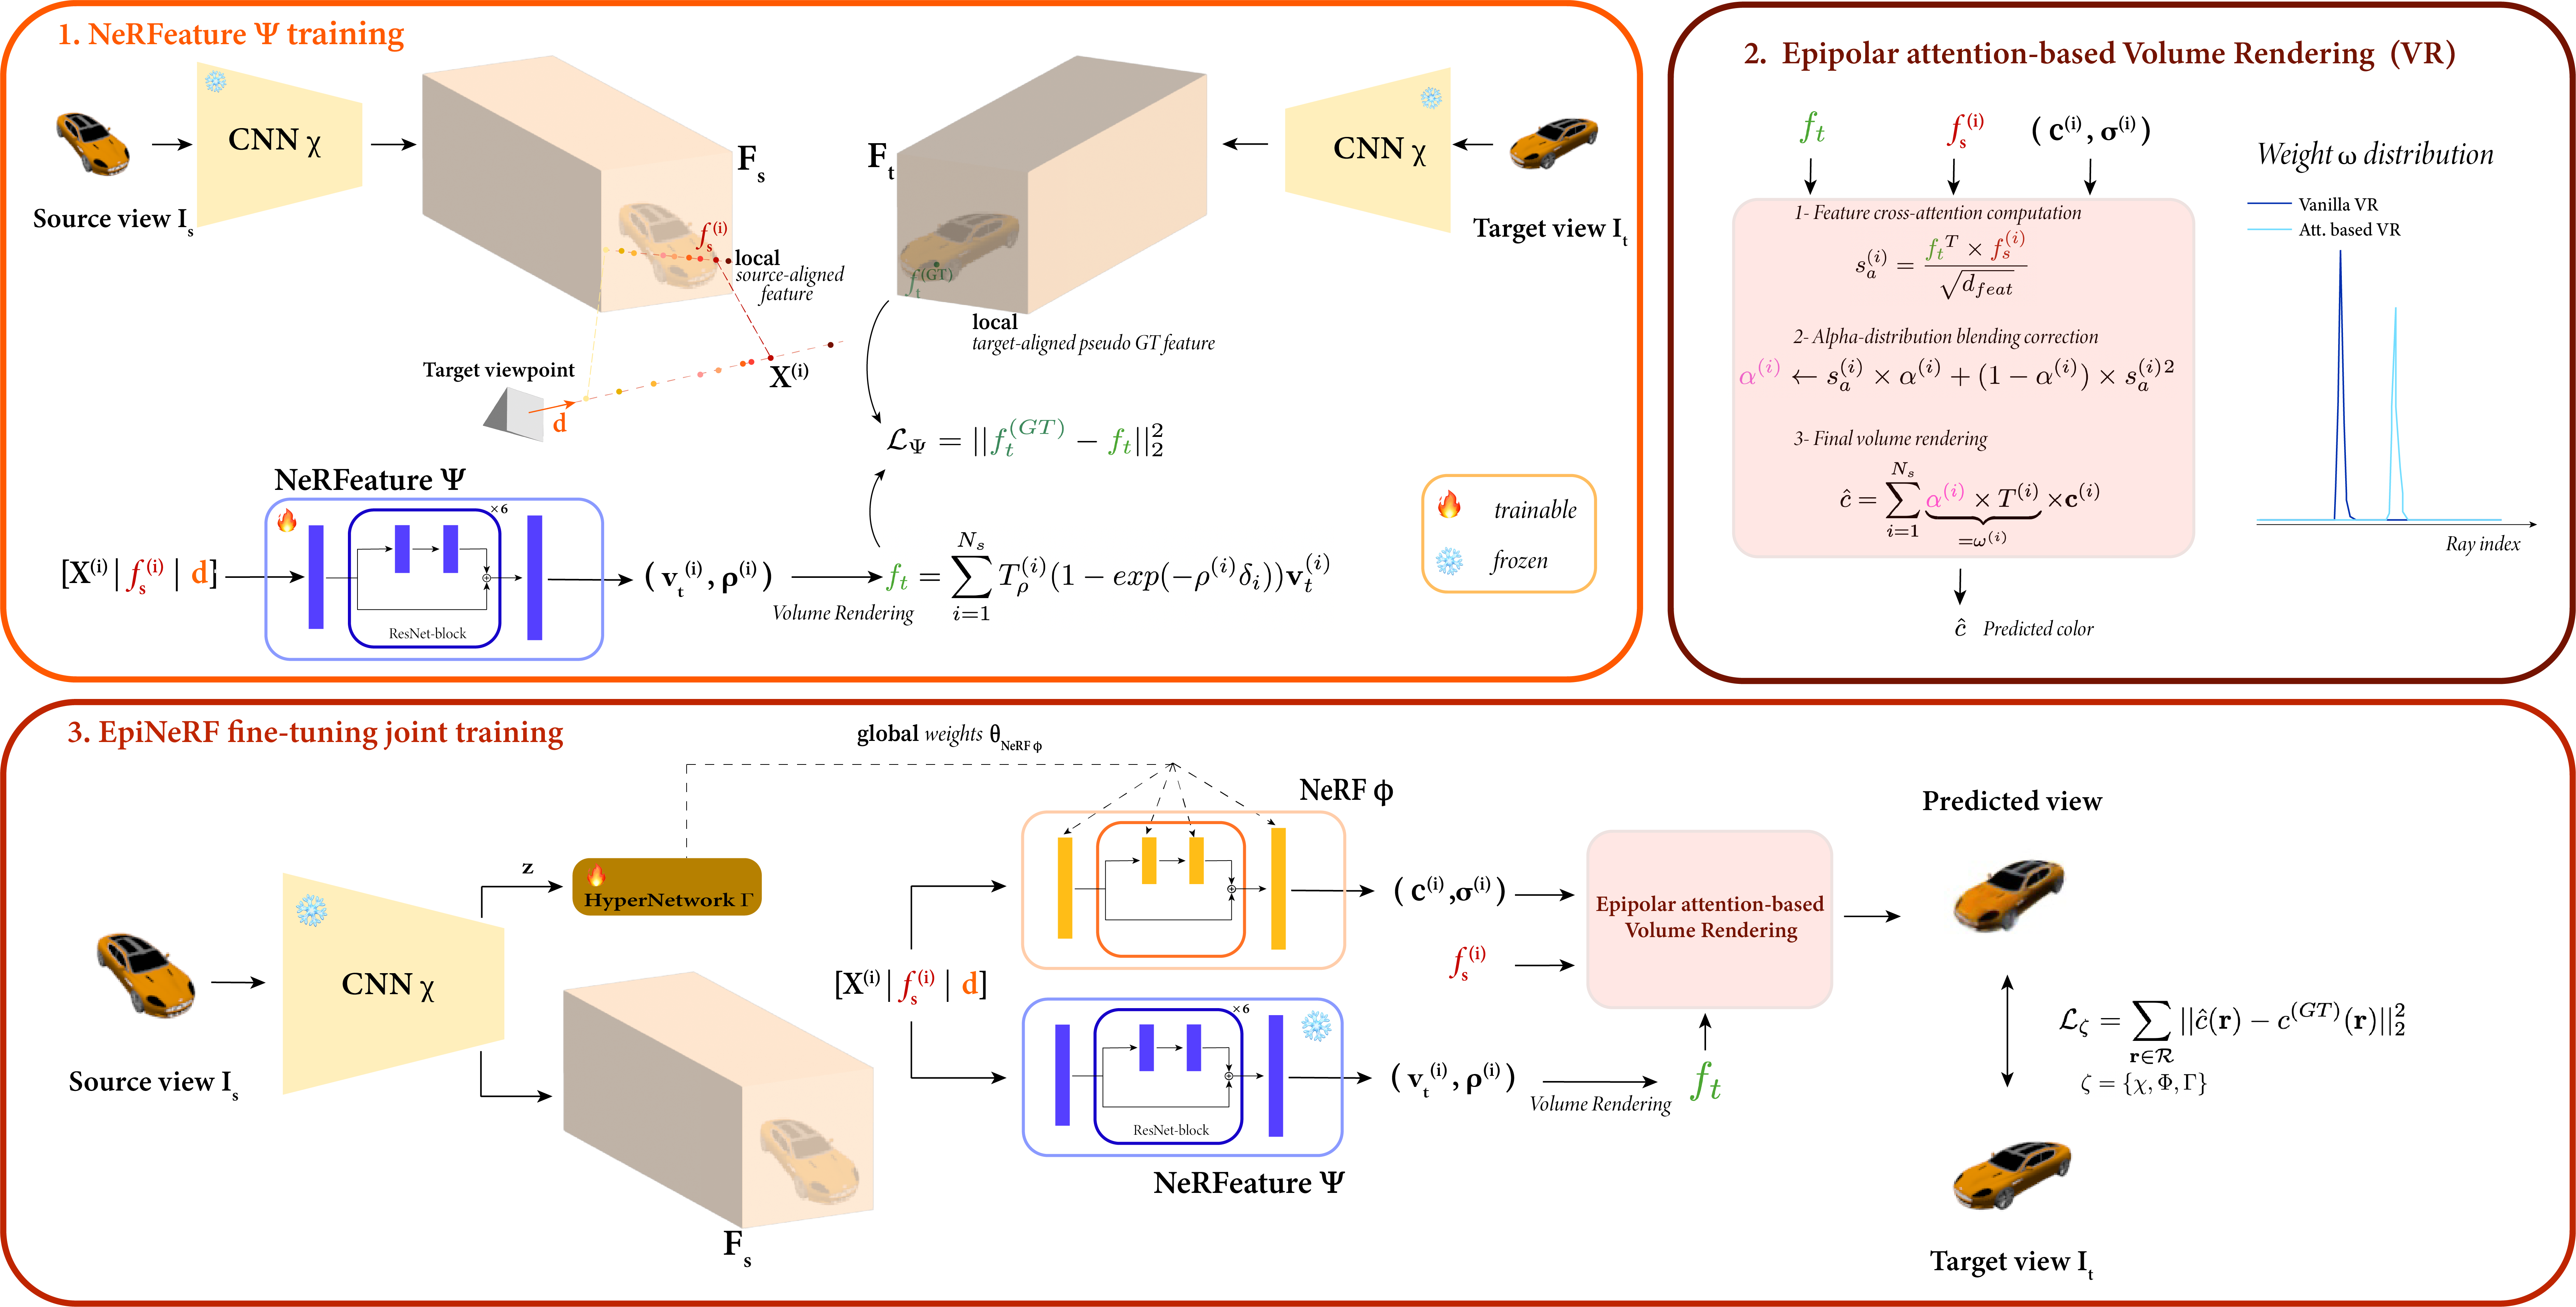
\includegraphics[width=\linewidth]{images/epinerf/overview_architecture_NEW.png}
  \end{center}
  \caption{\textbf{Overview of our complete EpiNeRF architecture.} \textit{(Top left)} A pre-trained \ac{CNN} $\chi$ is used as teacher model to instruct a NeRF student model $\Psi$, termed NeRFeature, to generate deep features from any target viewpoint. \textit{(Top right)} Given the predicted target-aligned feature from $\Psi$, a light cross-attention score distribution is computed with all the source-aligned features to correct the weights sampling distribution. It forms our epipolar attention-based model. \textit{(Bottom)} EpiNeRF is finally fine-tuned with the epipolar attention-based mechanism, that adjusts the volume rendering equation through $\Psi$.}
  \label{fig:overview}
\end{figure*}

\subsection{NeRFeature: learn target-aligned features}
\label{subsec:nerfeature}

Feature volumes produced by 2D models, such as \ac{CNN} or \ac{ViT}, are inherently aligned with the RGB image they were trained on (\ie the source image $I_s$). We propose to distill such a feature space into 3D using a neural feature radiance field, termed NeRFeature $\Psi$. As depicted on the \textit{top-left} panel of Figure \ref{fig:overview}, a pretrained teacher 2D \ac{CNN} encoder $\chi$ produces \textit{pseudo} ground truth features from the target viewpoint. One could also retrain such a \ac{CNN} from scratch with a proper image-conditioned RGB \ac{NeRF} architecture, as \citep{yu2021pixelnerf,li2022symmnerf,lin2023vision,jang2021codenerf} did in their work. These features are then used to supervise the distillation training of the 3D NeRFeature $\Psi$. \newline

For any 3D point $\mathbf{X}^{(i)}$ expressed in the world coordinate system along a ray $\mathbf{r}$ from a target direction $\mathbf{d}$, we denote: 

\begin{equation}
    f_{s}^{(i)} = \mathbf{F}_{s}(\pi(\mathbf{X}^{(i)}))  \in \mathbb{R}^{d_{\text{feat}}} 
    \label{eq:projection}
\end{equation}

the source-aligned feature that was extracted from $\mathbf{F}_{s}=\chi(I_{s})$ through the perspective projection $\pi$ of $\mathbf{X}^{(i)}$ on the feature plane.

As $\Psi$ must be generalizable (\textit{i.e} render meaningful features for unseen objects or scene), NeRFeature has to be conditioned with such an source oriented feature $f_{s}^{(i)}$. The complete formulation for $\Psi$ is therefore given by:

\begin{equation}
    \Psi(\mathbf{x}^{(i)},\mathbf{d},f_{s}^{(i)}) = (\rho^{(i)},\mathbf{v}_{t}^{(i)}) \in \mathbb{R}_{+}\times \mathbb{R}^{d_{\text{feat}}}
\end{equation}

The target-aligned feature $\mathbf{f}_{t}$ is obtained through the vanilla volume rendering equation, which is computed over the $N_s$ sampled points on \textbf{r}, as expressed in Equation \eqref{eq:main_nerf}.

This learned feature field is queried during the fine-tuning phase (see \textit{bottom} part of Figure \ref{fig:overview} ) to render the target-aligned features used in our epipolar attention-based volume rendering mechanism (see Section \ref{subsec:epipolar_att}). 

\subsection{Feature-based epipolar attention}
\label{subsec:epipolar_att}

Once deep features from $\chi$ has been distilled into the NeRFeature $\Psi$, target-aligned features can be synthesized using only a source-aligned feature. 

Target-aligned $\mathbf{f}_{t}$ (\textit{key} \textbf{k}) and source-aligned features $\mathbf{f}_{s}^{(i)}$(\textit{queries} \textbf{q}) form a light the cross-attention \citep{vaswani2017attention} $\mathbf{s}_{a}^{(i)}$ score:

\begin{equation}
    s_{a}^{(i)} = \frac{\mathbf{q}^{T}\mathbf{k}}{\sqrt{d_{\text{feat}}}}= \frac{f_{t}^{T}\times f_{s}^{(i)}}{\sqrt{d_{\text{feat}}}}
\label{eq:attention}
\end{equation}

All source-aligned features lie on the epipolar line defined by the sampled pixel in the target view. We denote:

\begin{equation}
  \mathbf{s}_{a} = \{ s_{a}^{(i)}\}_{i=1}^{N_{s}}
\end{equation}
 the entire distribution over the $N_s$ samples drawn along the ray $\mathbf{r}$. The attention distribution is then directly involved into the rendering process through the following $\alpha$-blending: 

\begin{equation}
\label{eq:alpha}
\alpha  \gets \textbf{s}_{a}\alpha + (1-\alpha)\textbf{s}_{a}^{2}
\end{equation}

The annex section \ref{appendix:epinerf-feature} gives additional information regarding how and why such a cross-attention distribution needs to be normalized and adjusted using sigmoid functions before getting involved in any volume rendering procedure. Our complete feature epipolar attention-based module is shown in the \textit{top-right} block of Figure \ref{fig:overview}. 

As implicly defined earlier in Equation \eqref{eq:weights}, the attention-based correction to $\alpha$ directly affects the transmittance \textbf{T}, as it corresponds to the cumulative product of the $1 - \alpha^{(j)}$ terms. The Figure \ref{fig:overall_attention} illustrates how both transmittance and $\alpha$ distributions shift the final weight distribution. 

\begin{figure}[h!]
    \begin{center}
  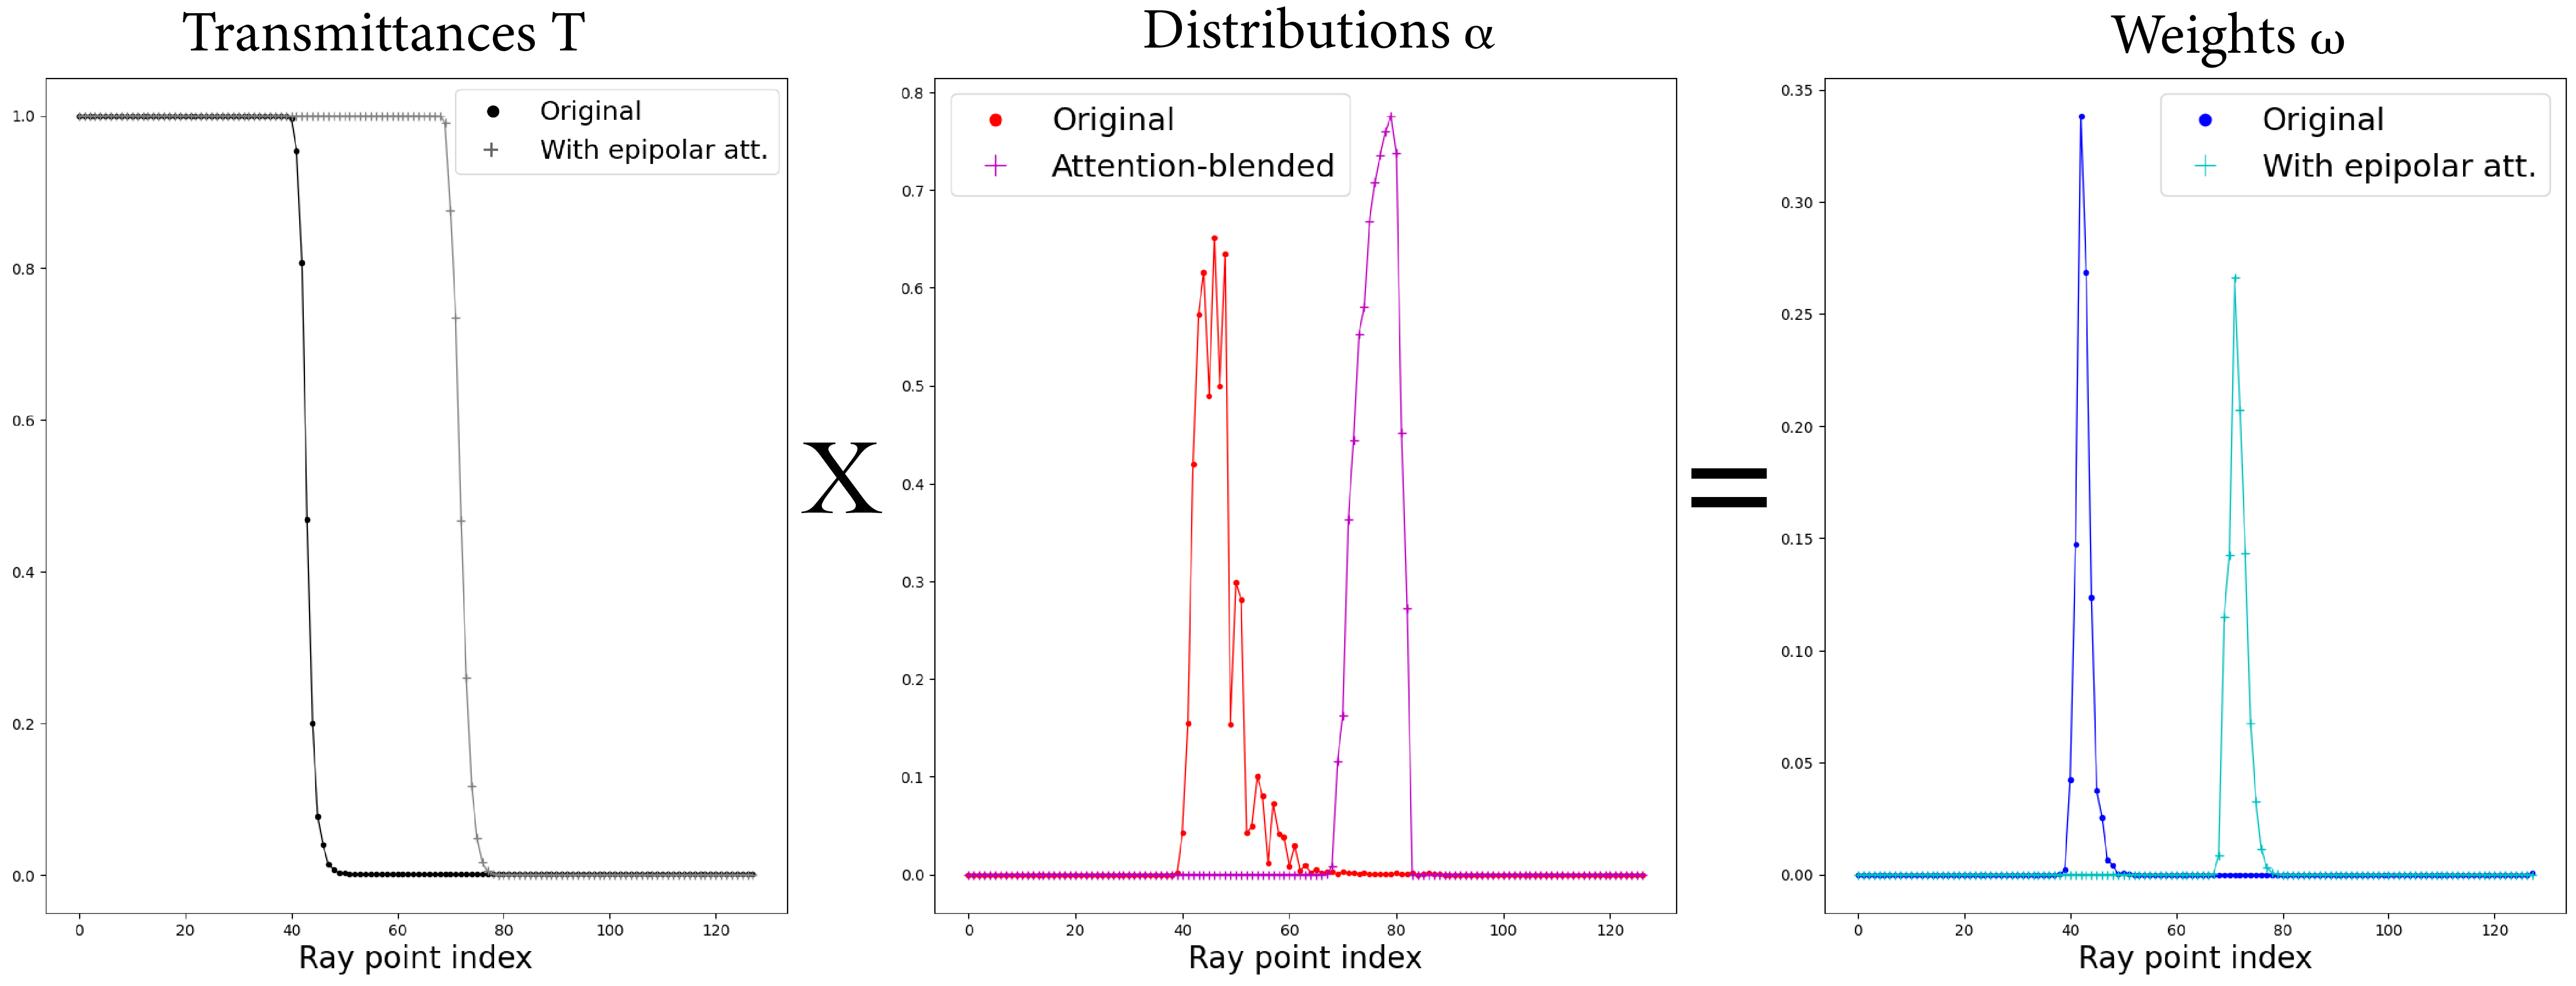
\includegraphics[width=\linewidth]{images/epinerf/SUPP_VR_OVERLEAF.png}
  \caption{\textbf{Influence of our epipolar attention mechanism over the volume rendering equation.} As the $\alpha$ distribution has been blended with the cross-attention distribution from NeRFeature $\Psi$, transmittance $T$ is naturally affected as well. Final weight composite distribution is thus corrected during the volume rendering process.} 
  \label{fig:overall_attention}
  \end{center}
\end{figure}

The attention distribution $\textbf{s}_{a}$ impact on the coarse and fine \ac{NeRF} networks is twofold. It directly influences the weight sampling during volume rendering for the coarse \ac{NeRF} but also improves sample locations for the fine \ac{NeRF} through the hierarchical sampling. Details on the impact of our feature-based epipolar cross attention during volume rendering can be found in Section \ref{subsec:visual_insights} and Figure \ref{fig:attention_overview}.  

\subsection{EpiNeRF: the complete architecture}
\label{subsec:epinerf}

\noindent\textbf{Source-aligned features with the CNN $\chi$.} Plethora of recent \ac{NeRF}-based \ac{NVS} works leverage their radiance field on a source-aligned feature volume $\mathbf{F}_{s}$, obtained from either a CNN ~\citep{jang2021codenerf,yu2021pixelnerf,li2022symmnerf} or a \ac{ViT} ~\citep{lin2023vision}. However, intermediate features produced by the inner encoder are often fused and upscaled in a vanilla way, through bilinear upsampling and concatenation operations in the \ac{CNN} decoder. 

The source-aligned feature volume can be built differently, by accounting on residual connections and atrous convolutions, as ~\citep{chan2023genvs} did. 
EpiNeRF thus rather gets consideration for DeepLabV3+~\citep{chen2018encoder} backbone decoder to produce $\textbf{F}_{s}\in \mathbb{R}^{d_{\text{feat}} \times H \times W}$. Since our feature volume $\textbf{F}_{s}$ matches the resolution of the input image $\mathbf{I}_s$, it enables more precise projection and feature sampling. An overview of the two different feature fusion strategies is illustrated in Figure \ref{fig:feature_encoder}. 

\begin{figure}[h!]
  \begin{center}
  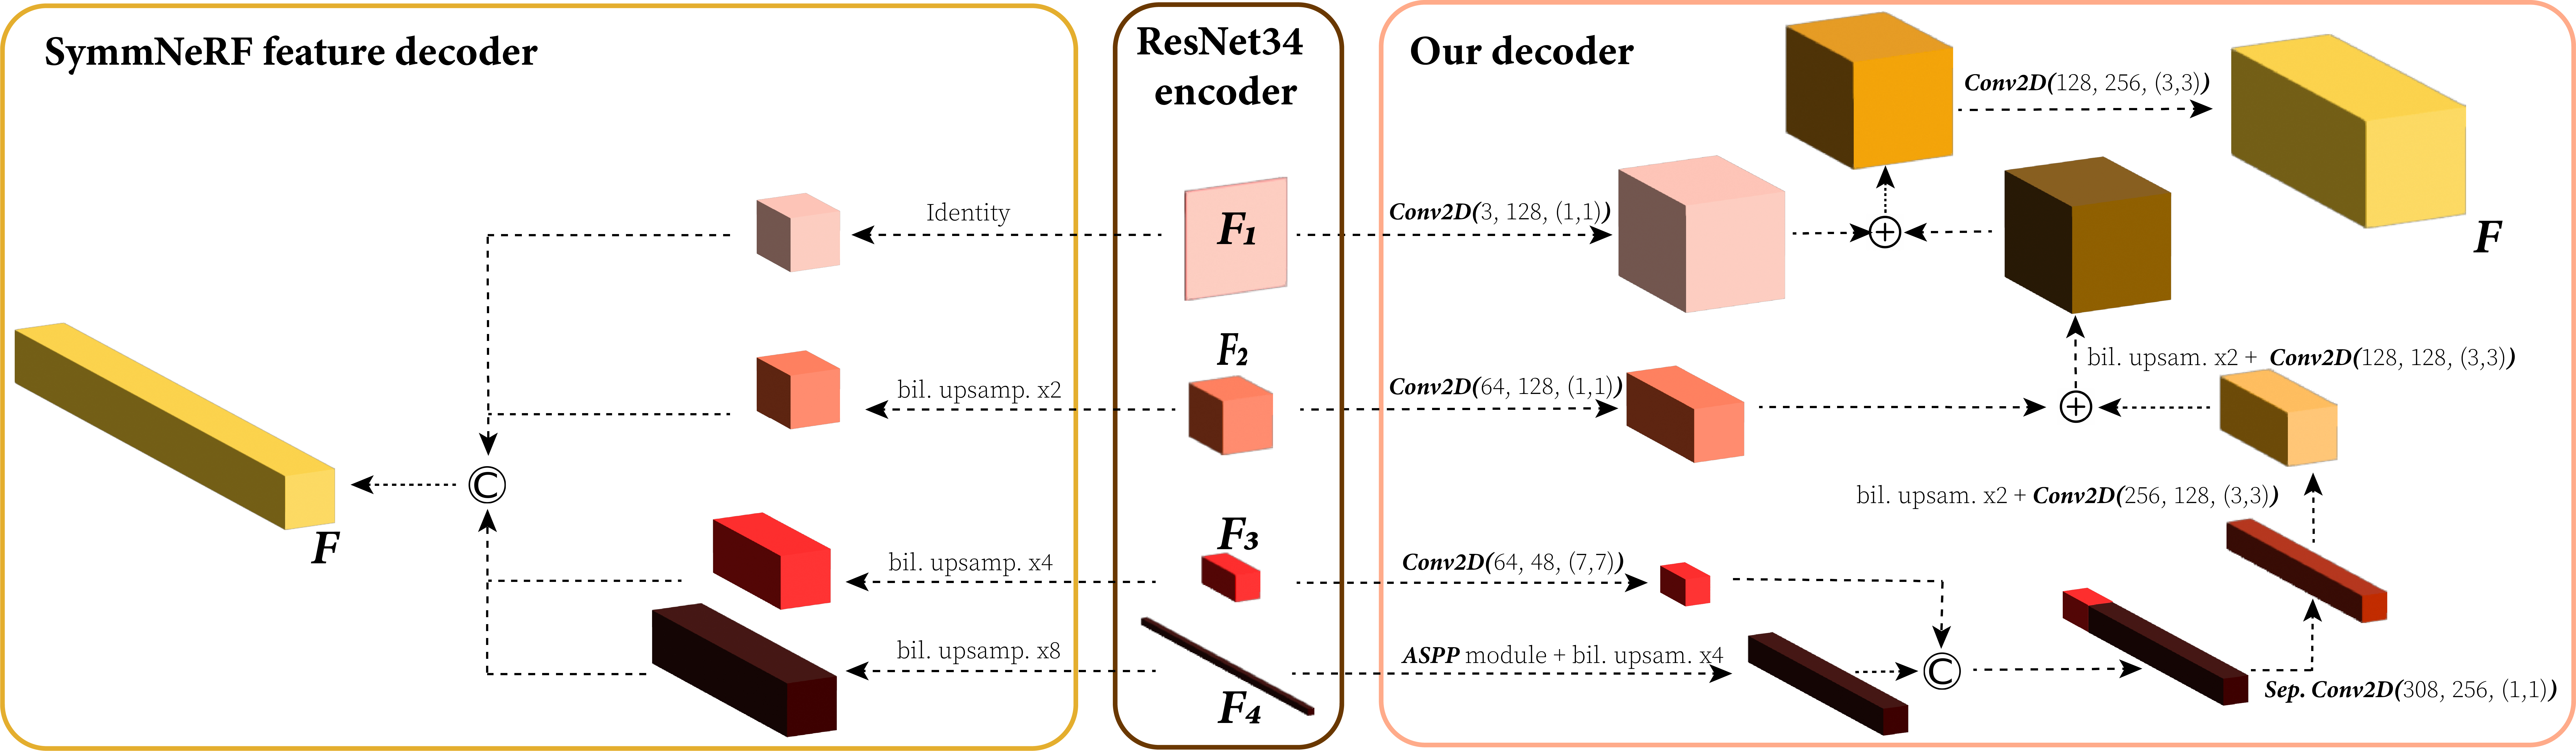
\includegraphics[width=\linewidth]{images/epinerf/feature_fusion_encoder.png}
  \end{center}
     \caption{\textbf{Comparison of the CNN decoder $\chi$ from SymmNeRF (left) and ours DeepLabV3+ (right).} CNN $\chi$ in both case leverages a ResNet34-based encoder ~\citep{he2016deep}. }
  \label{fig:feature_encoder}
  \end{figure}


\noindent\textbf{Symmetry prior integration.}
  Following SymmNeRF ~\citep{li2022symmnerf} prior work, we make the assumption that the (YZ) plane in the canonical coordinates system is a symmetry plane for the implicit 3D scenes we are aiming to reconstruct. A 3D point $\mathbf{X}^{(i)}$ along a target ray \textbf{r} has a symmetrical point with respect to the (YZ)-symmetry plane through:
  \begin{equation}
      \mathbf{X}^{(i)}_{symm} = \mathbf{M}\mathbf{X}^{(i)}
  \end{equation}
  where $\mathbf{M} = \mathbf{I}_{4}\footnote{the Identity matrix in $\mathbb{R}^{4}$} - 2e_{1}e_{1}^{T}$ and $e_{1}$ is the first 3D unit basis vector. This symmetrical 3D point is back-projected on the same source-aligned feature volume $\mathbf{F}_{s}$ produced by $\chi$ from $I_s$. The local deep feature fed to the NeRF $\Phi$ is finally the concatenation, noted $[.|.]$, of these two source-aligned features: 
  \begin{equation}
      f^{(i)} = \left[f_{s}^{(i)} | f_{s,symm}^{(i)}\right]
  \end{equation}

\noindent\textbf{Local and global NeRF conditioning.} The ResNet34 encoder from $\chi$ primarily produces an intermediate set of features $(\mathbf{F}_{1},\mathbf{F}_{2},\mathbf{F}_{3},\mathbf{F}_{4})$ from $\textbf{I}_{s}$ (see Figure \ref{fig:feature_encoder}). While $\mathbf{F}_{s}$ must be considering as a local input conditioning of the radiance field (since feature are pixel-wise sampled during the perspective projection), we leveraged on an additional \ac{MLP} network, called a hypernetwork $\Gamma$. Following prior works \citep{sitzmann2019scene,li2022symmnerf}, $\Gamma$ is intended to learn the RGB radiance field weights $\theta_{NeRF_{\Phi}}$ during training. It takes as input a latent code $\mathbf{z}$, obtained from a non-linear projection of the deepest feature $\mathbf{F}_{4}$:

\begin{equation}
  \Gamma(\mathbf{z}) = \theta_{NeRF_{\Phi}} 
\end{equation}

The complete output of our \ac{CNN} encoder-decoder $\chi$ can thus be re-written as:

\begin{equation}
    \textbf{z}, \textbf{F}_{s} = \chi(I_{s})
\end{equation}

Figure \ref{fig:supp_hyper_nerf} shows the architecture of the hypernetwork $\Gamma$ and how such an MLP interacts with the RGB NeRF $\Phi$.

\begin{figure}[htp!]
  \begin{center}
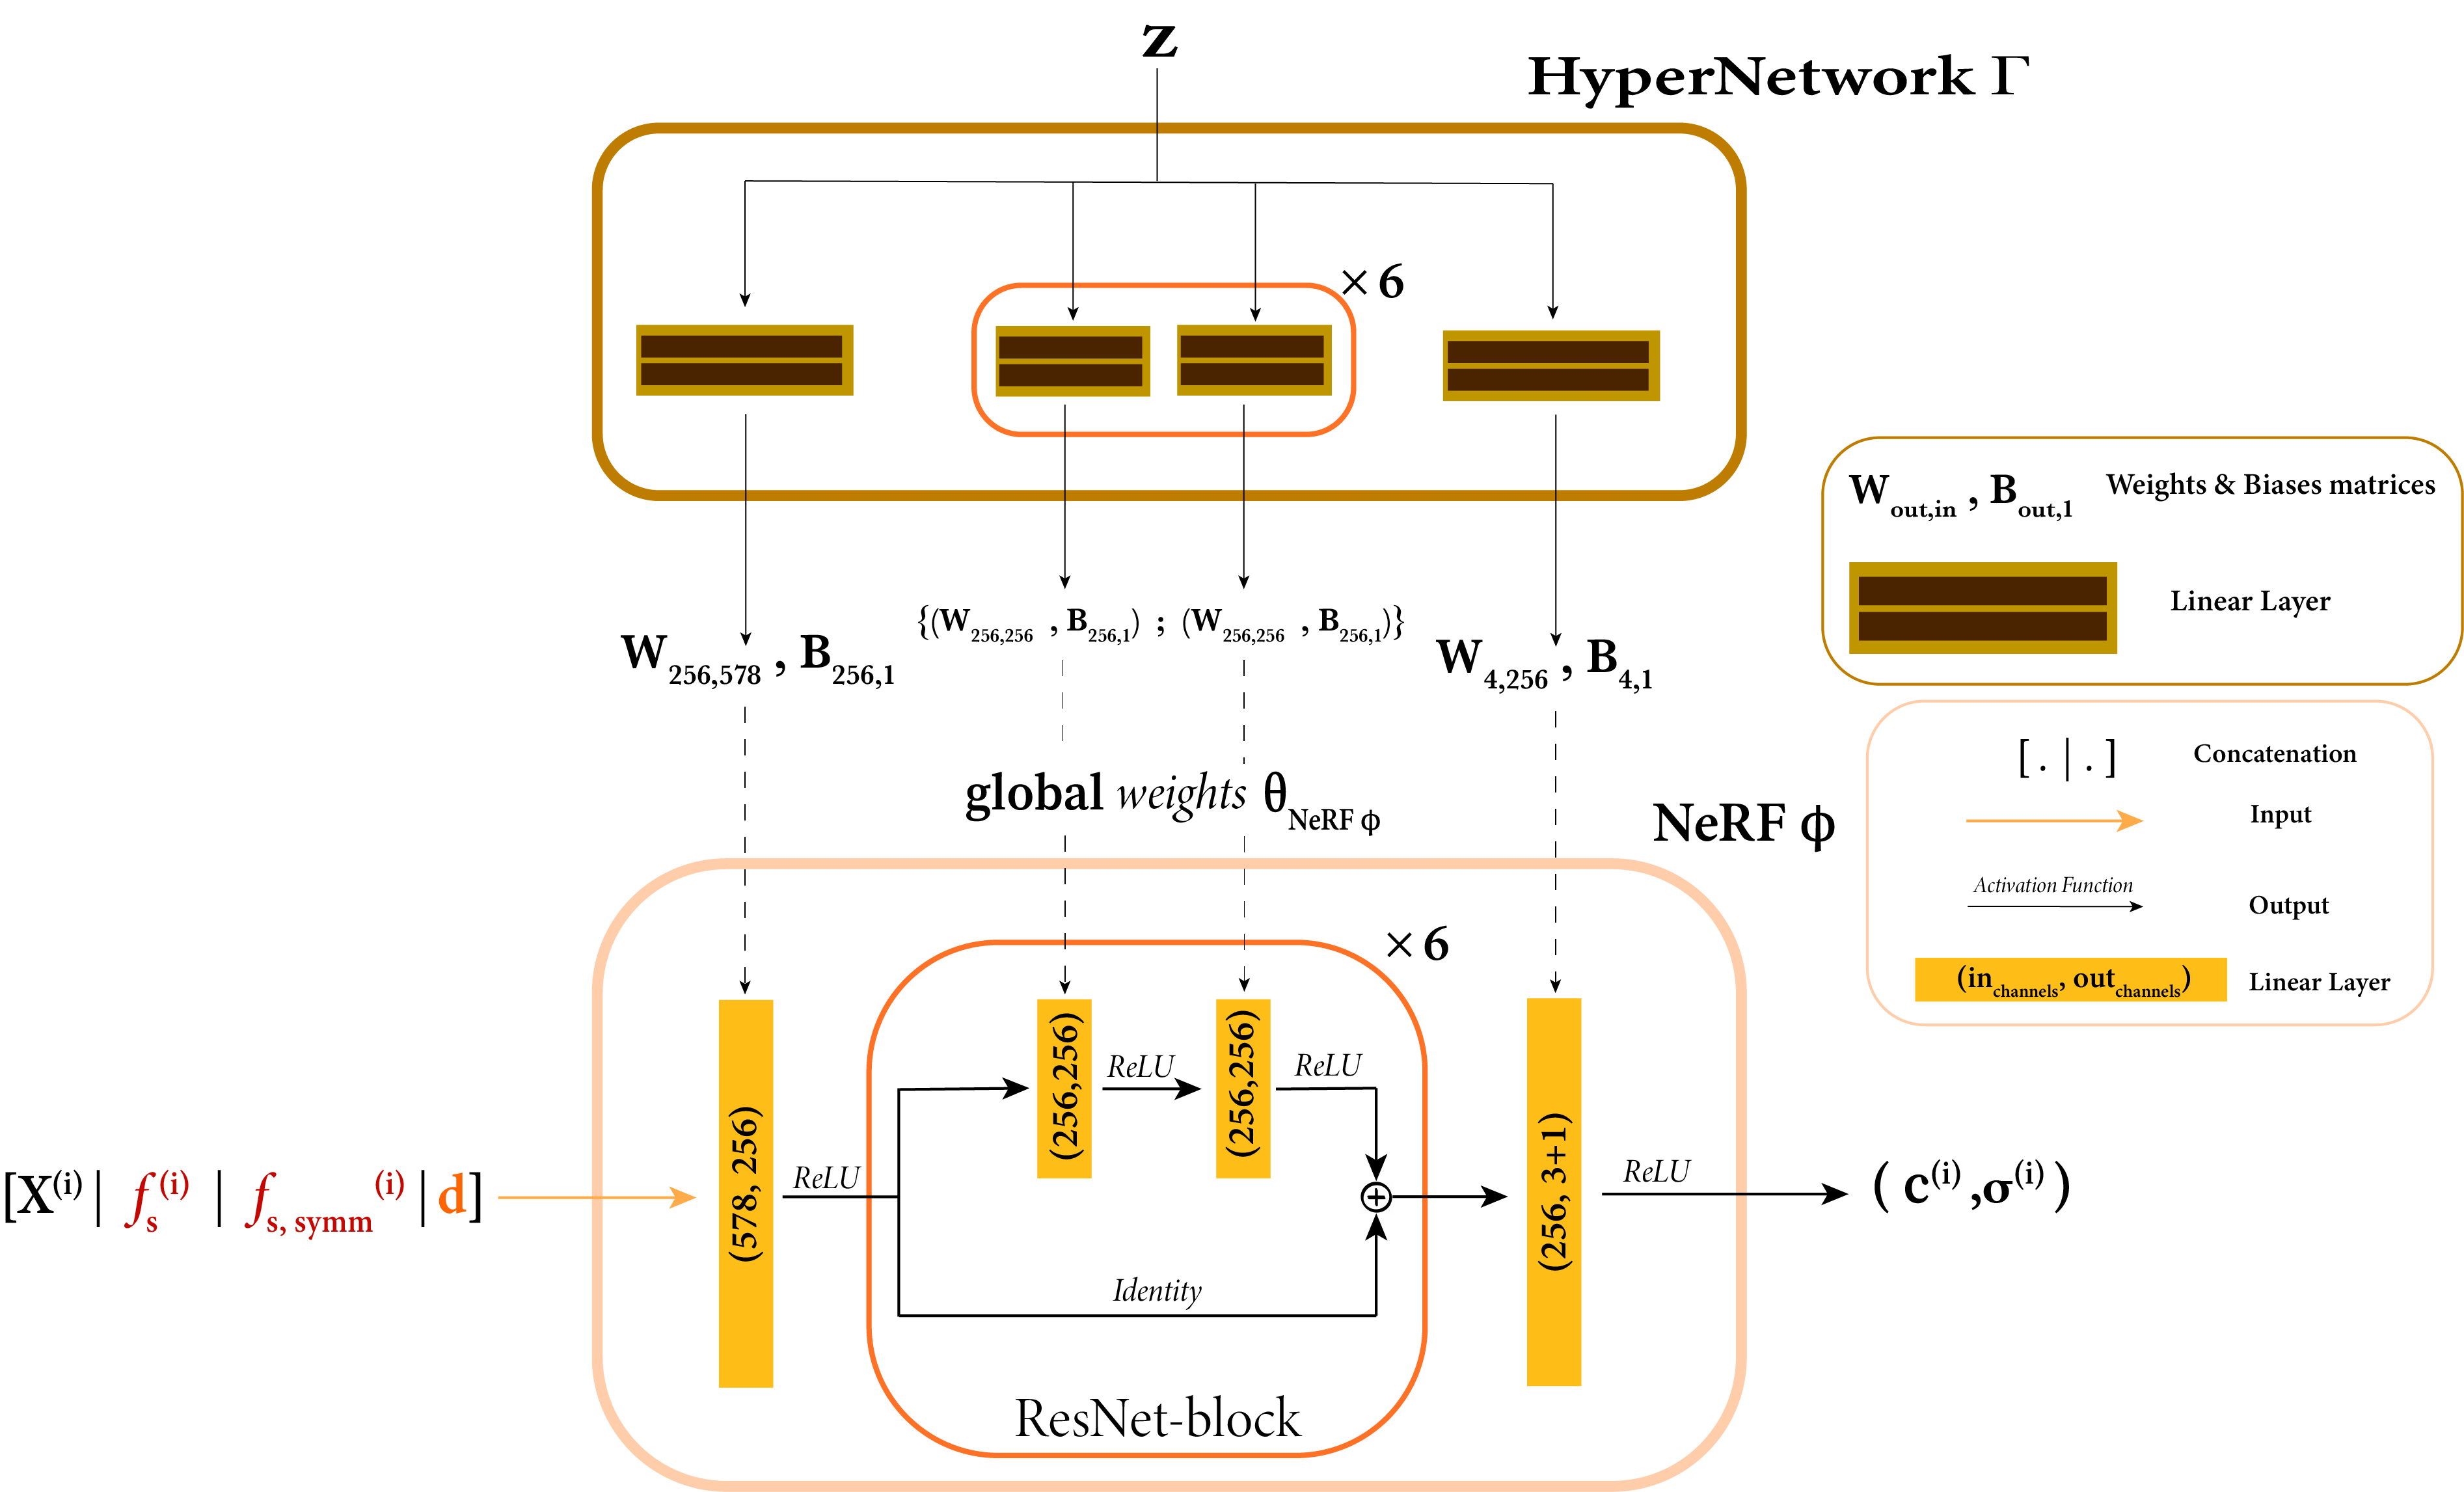
\includegraphics[width=\linewidth]{images/epinerf/supp_hyper_nerf.png}
\caption{\textbf{Complete overview of NeRF $\phi$ architecture.} The hyperNetwork $\Gamma$ is trained to predict the finite set of weights for $\Phi$. It indirectly acts as a global conditioning of the radiance field, in addition to the direct local conditioning offered by the source-aligned pixel-wise feature $f_{s}^{(i)},f_{s,symm}^{(i)}$.}
\label{fig:supp_hyper_nerf}
\end{center}
\end{figure} 

The term $\theta_{NeRF_{\Phi}}$ represents a finite set of weight and bias matrices that $\Gamma$ learns to predict based on the deep latent code $\mathbf{z}$. By introducing this hypernetwork to predict the \ac{NeRF}'s weights $\theta_{NeRF_{\Phi}}$, $\Phi$ is globally conditioned, in addition to the local conditioning provided by the source aligned features.  \newline

Primary role of $\Gamma$ is therefore to model NeRF's weights $\theta_{NeRF_{\Phi}}$ distribution according to a single source viewpoint. Hypernetwork $\Gamma$ does not have to be trained with a specific loss objective: its weights are updated during  backpropagation through the vanilla $\mathcal{L}_{2}$ loss function defined over the sampled RGB pixels. Additional information on the entire training procedure can be found in appendix \ref{appendix:epinerf-training}. 

The main NeRF $\Phi$ in our EpiNeRF architecture is thus both locally (on its input) and  globally (through its weights) conditioned: 
\begin{equation}
     \Phi_{\theta}(\mathbf{x}^{(i)},\mathbf{d},f_{s}^{(i)},f_{s,symm}^{(i)},f_{t}) = (\sigma^{(i)},\mathbf{c}^{(i)}) \hspace{.5cm}\text{;}\hspace{.5cm}  \theta = \Gamma(\mathbf{z})
\end{equation}

\noindent\textbf{Training.} As shown in Figure \ref{fig:overview}, our EpiNeRF architecture has a multi-stage training strategy. It integrates a feature radiance field, termed NeRFeature $\Psi$, in combination with a CNN-based encoder-decoder $\chi$ that condition the main RGB radiance fields $\Phi$ through an epipolar based attention mechanism. A hypernetwork $\Gamma$ also globally conditions $\Phi$, by predicting its learnable parameters through a lightweight \ac{MLP}. 

Considering a training set of N objects $\{\mathcal{D}\}_{i=1}^{N}$ with V different viewpoints $\mathcal{D}^{(i)} = \{I_{i}^{(j)},\pi_{i}^{(j)}\}_{j=1}^{V}$ per instance and a batch of rays $\mathcal{R}$, EpiNeRF is optimised through the loss functions: 
\begin{equation}
\label{eq:nerfeature_loss}
\begin{split}
 \min_{\Psi} \sum_{i}\sum_{j}\mathcal{L}_{\Psi}\left(I_{i}^{(j)},\pi_{i}^{(j)},\Psi,\chi \right) \hspace{.2cm} \\ \hspace{.2cm}\mathcal{L}_{\Psi}= \sum_{\mathbf{r}\in\mathcal{R}} || f_{t}(\mathbf{r}) - f_{t}^{(GT)}(\mathbf{r}) ||_{2}^{2}
\end{split}
\end{equation}
and 
\begin{equation}
\label{eq:epinerf_loss}
\begin{split}
 \min_{\zeta=\{\chi,\Phi,\Gamma\}}\sum_{i}\sum_{j}\mathcal{L}_{\zeta}\left(I_{i}^{(j)},\pi_{i}^{(j)},\Psi,\zeta \right)\hspace{.2cm}  \\ \hspace{.2cm}\mathcal{L}_{\zeta}= \sum_{\mathbf{r}\in\mathcal{R}} || \hat{c}(\mathbf{r}) - c^{(GT)}(\mathbf{r}) ||_{2}^{2}
\end{split}
\end{equation}


where $c^{(GT)}(\mathbf{r})$ represents the ground truth pixel that was sampled on $\mathbf{I}_{t}$, and $f^{(GT)}(\mathbf{r})$ the \textit{pseudo} ground truth target-aligned feature that was sampled from $F_{t}=\chi(I_{t})$. Deep features produced by NeRFeature are implicitly conditioned by $\chi$ since the source aligned feature $f_s^{(i)}$ is fed as input. A full and explicit formulation of these losses  is provided in appendix \ref{appendix:epinerf-training}. 

\section{Experiments}
\label{subsec:epinerf/experiments}
\subsection{View synthesis on synthetic data - SRN ShapeNet}
The presented results are obtained using the ShapeNet dataset~\citep{chang2015shapenet}, specifically focusing on the ShapeNet-SRN~\citep{sitzmann2019scene} version. The \textit{Cars} class contains 3,514 objects, and the \textit{Chairs} class has 6,591. Training is conducted using 50 different views per instance, while the test set includes 251 views per object, sampled along an archimedean spiral.\newline

Our method achieves state-of-the-art performance, as shown in Table \ref{table:comp_res}, and even outperforms the heavier transformer-based architecture from ~\citep{lin2023vision} on nearly all metrics.

\begin{table}[h!]
\caption{\textbf{Quantitative results.} Comparisons against state-of-the-art methods on the category specific \textit{Chairs} and \textit{Cars} classes from the ShapeNet-SRN dataset. Best results are highlighted in \colorbox{red!25}{red}, second ones in \colorbox{orange!25}{orange} and third ones in \colorbox{yellow!25}{yellow}. }
\label{table:comp_res}
\begin{center}%\centering%
\begin{adjustbox}{width = \linewidth}
\begin{tabular}[h]{c||ccccccc}
\hline
 Method & \multicolumn{3}{c}{Cars} & \multicolumn{3}{c}{Chairs} \\
 &  SSIM ($\uparrow$) & PSNR ($\uparrow$) & LPIPS ($\downarrow$) & SSIM ($\uparrow$) & PSNR ($\uparrow$) & LPIPS ($\downarrow$)\\
\hline
SRN ~\citep{sitzmann2019scene}& \cellcolor{yellow!25}0.89 & 22.25 & 0.129 & 0.89 & 22.89 & 0.104\\
PixelNeRF ~\citep{yu2021pixelnerf} & \cellcolor{orange!25}0.90 & 23.17 & 0.146 & \cellcolor{yellow!25}0.91 & 23.72 & 0.128\\
FE-NVS ~\citep{guo2022fast} & \cellcolor{red!25}0.91 & 22.83 & \cellcolor{yellow!25}0.099 & \cellcolor{orange!25}0.92 & 23.21 & 0.077 \\
GeNVS~\citep{chan2023genvs}& \cellcolor{yellow!25}0.89 & 20.7 & 0.104 & - & - & - \\
ShaRF ~\citep{rematas2021sharf} & \cellcolor{orange!25}0.90 & 22.90 & - & \cellcolor{orange!25}0.92 & 23.37 & - \\
CodeNeRF ~\citep{jang2021codenerf} & \cellcolor{red!25}0.91 & \cellcolor{orange!25}23.80 & - & 0.90 & 23.66 & -  \\
SymmNeRF\footnotemark~\citep{li2022symmnerf}& \cellcolor{orange!25}0.90 & \cellcolor{yellow!25}23.10 & 0.110 & \cellcolor{yellow!25}0.91 & \cellcolor{yellow!25}24.14  & \cellcolor{orange!25}0.075 \\
VisionNeRF ~\citep{lin2023vision} & \cellcolor{red!25}0.91 & 22.88 & \cellcolor{red!25}0.084 & \cellcolor{red!25}0.93 & \cellcolor{orange!25}24.48  & \cellcolor{yellow!25}0.077 \\
Ours &\cellcolor{red!25} 0.91 & \cellcolor{red!25} 24.01  &\cellcolor{orange!25}  0.086 &  \cellcolor{orange!25}0.92   & \cellcolor{red!25}24.60&  \cellcolor{red!25}0.070 \\

\hline 
\end{tabular}
\end{adjustbox}
\end{center}
\end{table}
\footnotetext[2]{SymmNeRF results differ from the ones originally reported by authors since we had to retrain their architecture.}

As shown in Figures \ref{fig:exp-srn-cars} and \ref{fig:exp-srn-chairs}, EpiNeRF successfully combines the strengths of both SymmNeRF ~\citep{li2022symmnerf} and VisionNeRF~\citep{lin2023vision}. It renders novel views that are both sharp (eased by the \ac{ViT} in VisionNeRF) and consistent with symmetrical color patterns (enhanced by the symmetry prior in SymmNeRF). For instance, the gray stripe pattern in Figure \ref{fig:exp-srn-cars} (\textit{middle}) is  accurately synthesized by our architecture, unlike competing methods that either fail to produce sharp views (SymmNeRF) or to capture the inherent symmetrical band (VisionNeRF). 

\begin{figure}[h!]
    \begin{center}
  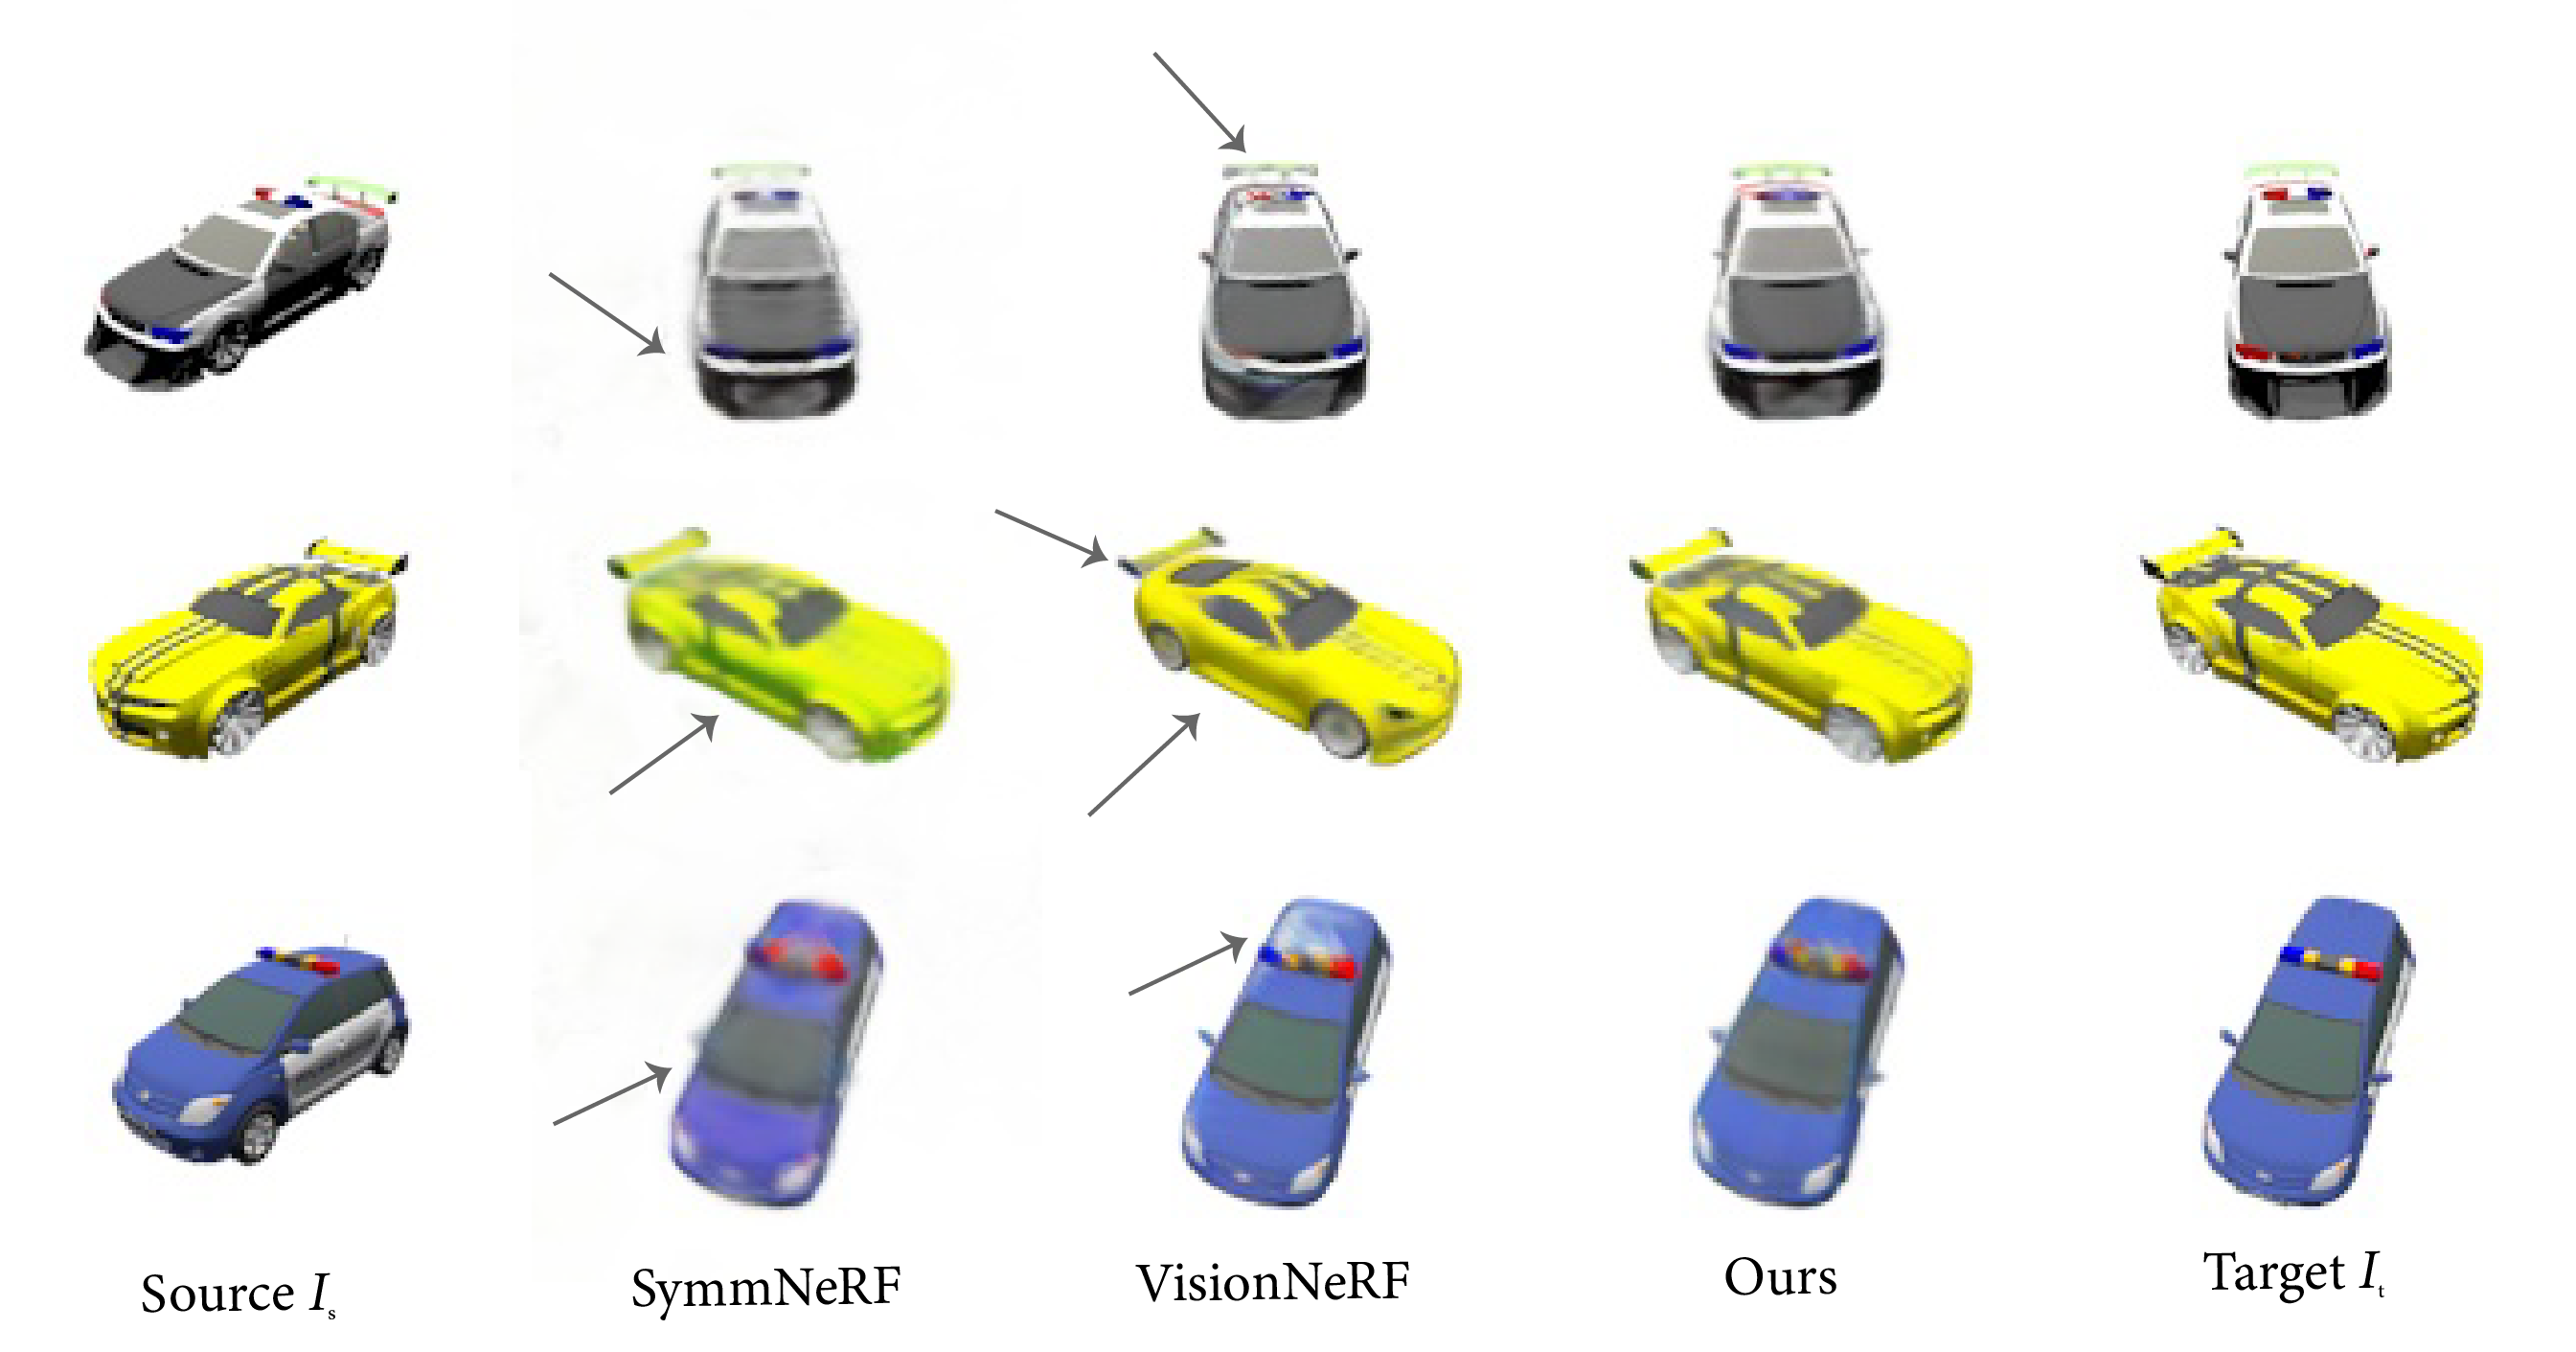
\includegraphics[width=\linewidth]{images/epinerf/cars_BMVC.png}
  \end{center}
  \caption{\textbf{Novel view synthesis on the ShapeNet category-specific} \textit{Cars}. Our method renders sharper novel views than SymmNeRF ~\citep{li2022symmnerf} while preserving the symmetry that VisionNeRF ~\citep{lin2023vision} fails to maintain.}
  \label{fig:exp-srn-cars}
\end{figure}

\begin{figure}[h!]
    \begin{center}
  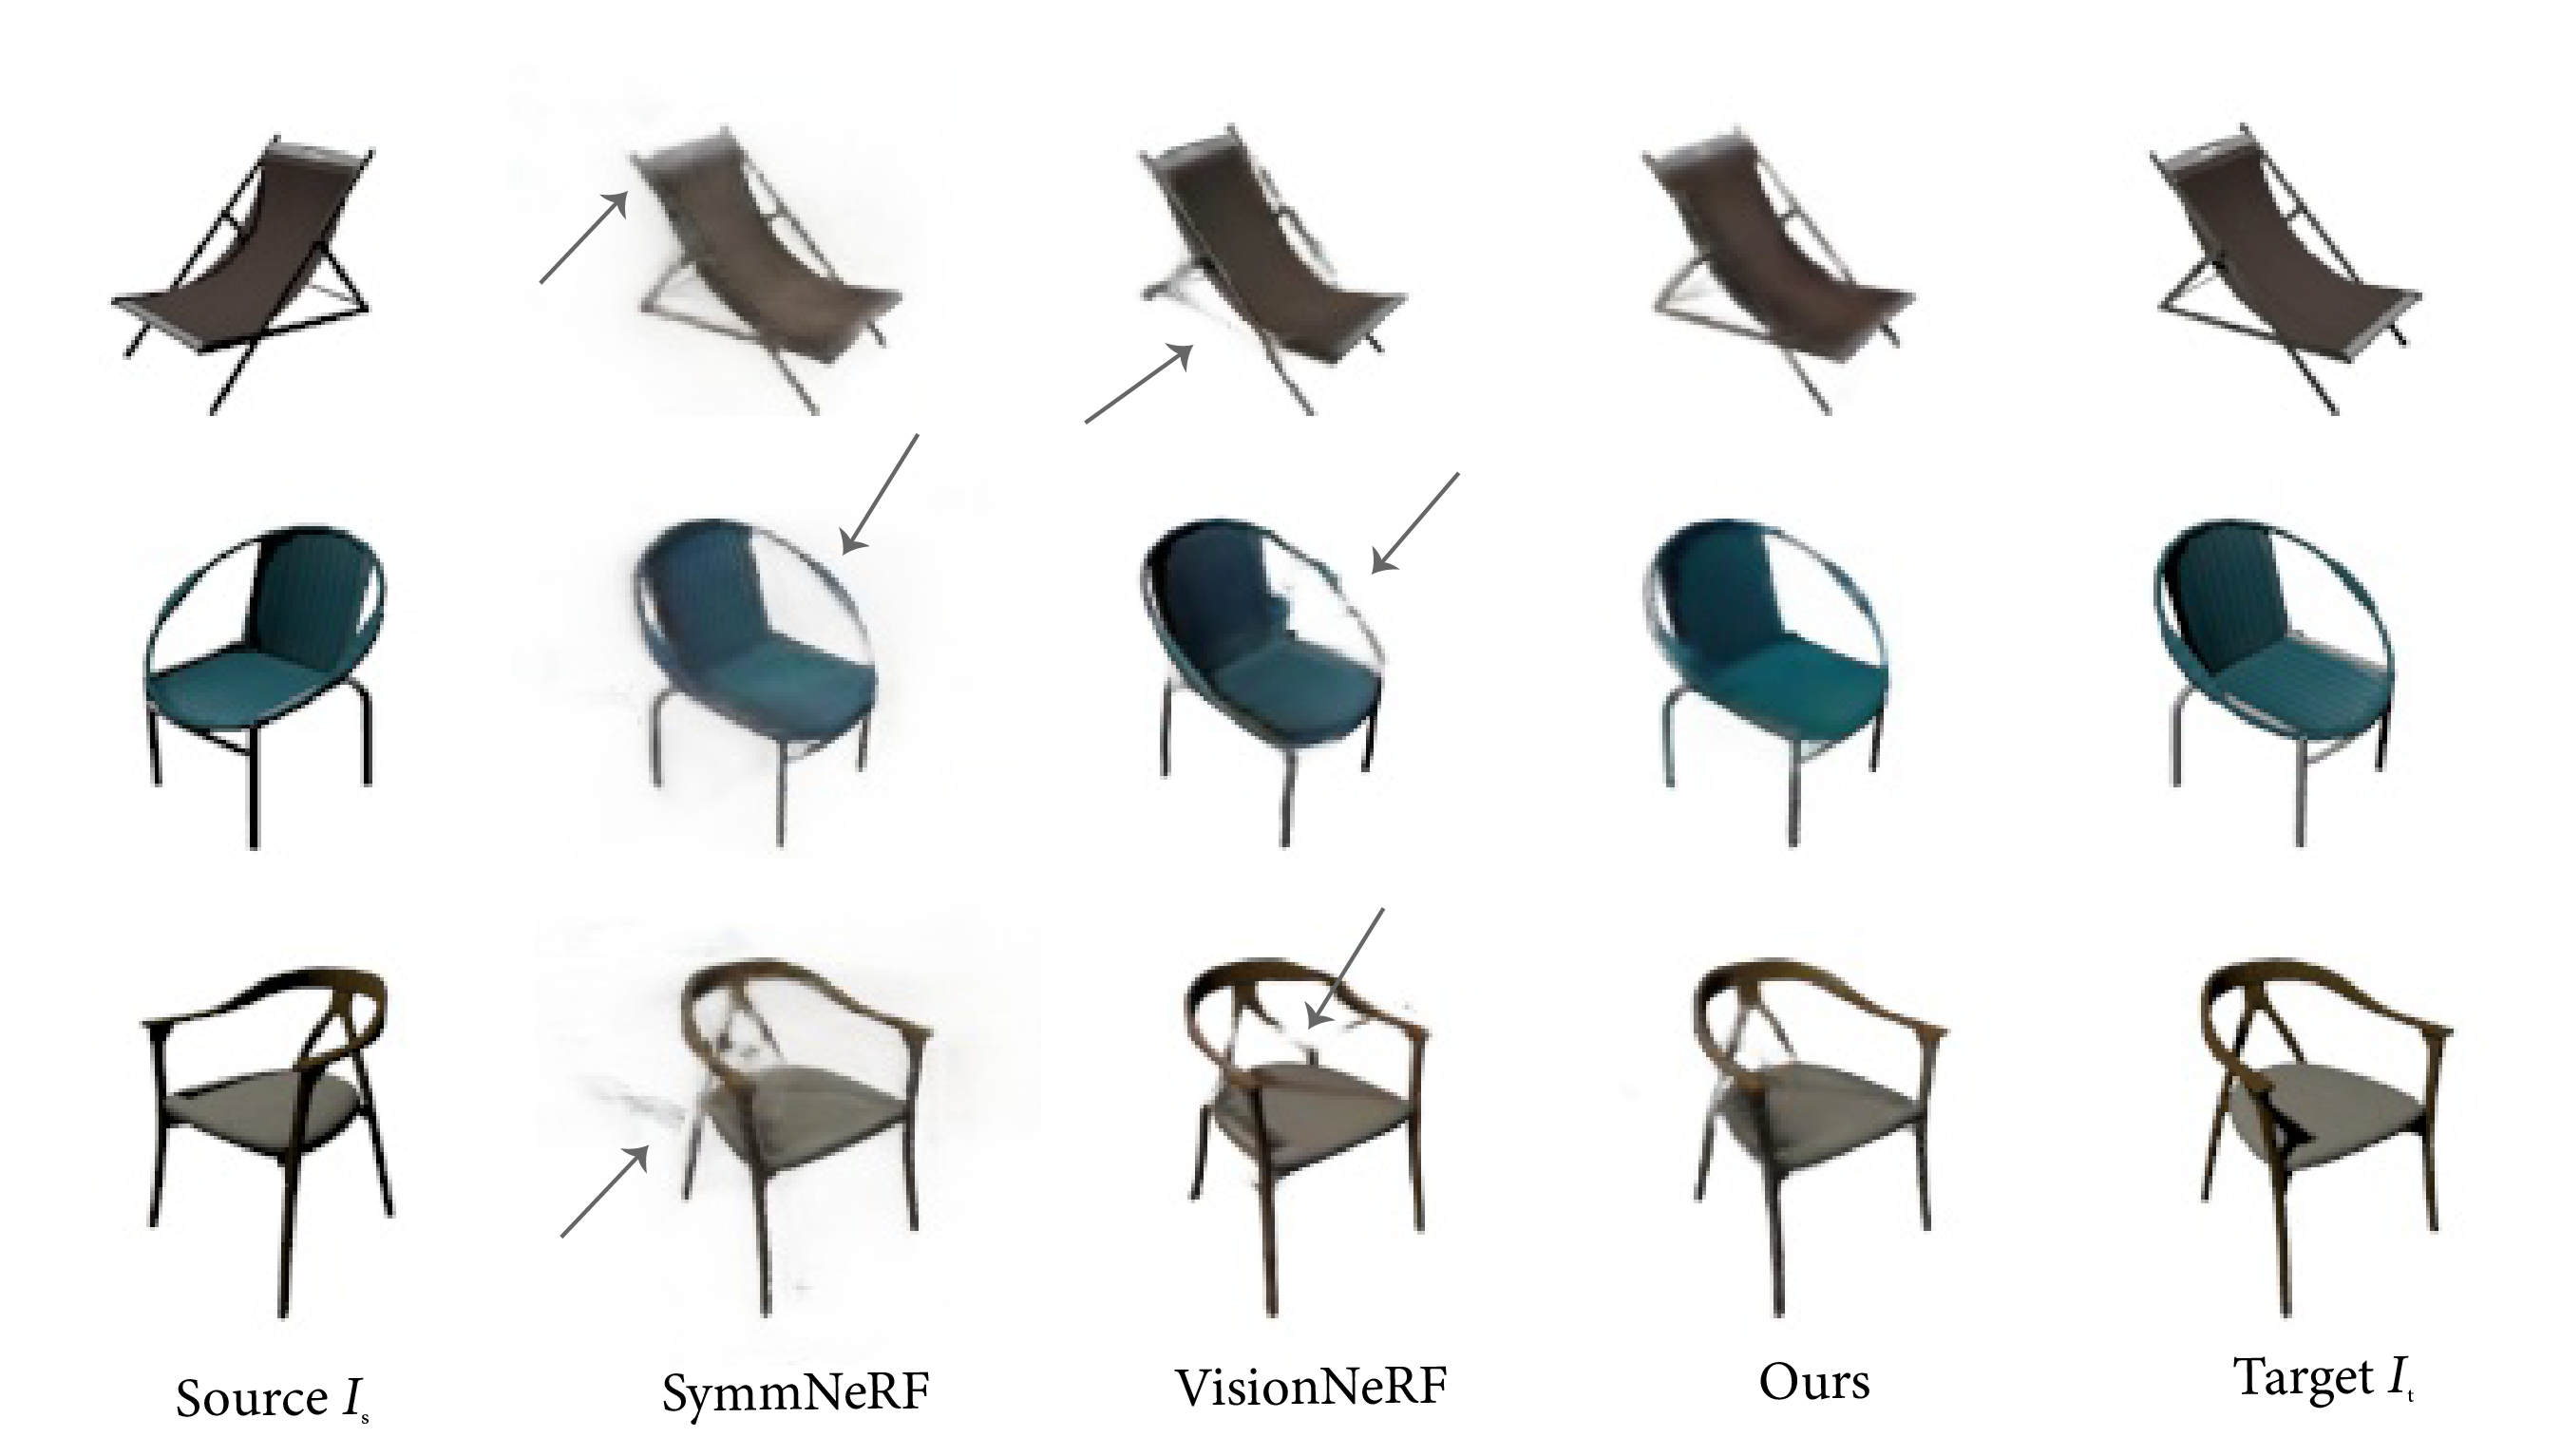
\includegraphics[width=\linewidth]{images/epinerf/chairs_BMVC.png}
  \end{center}
  \caption{\textbf{Novel view synthesis on the ShapeNet category-specific} \textit{Chairs}. Unlike EpiNeRF, both SymmNeRF \citep{li2022symmnerf} and VisionNeRF \citep{lin2023vision} fail to accurately render complex armrest structures.}
  \label{fig:exp-srn-chairs}
\end{figure}

Similar observations can be made for the \textit{Chairs} class in Figure \ref{fig:exp-srn-chairs}. VisionNeRF struggles to fully synthesize the intricate geometry of the back and armrests, failing to capture the chair's inherent symmetry. For instance, the armrest structure is partially missing in the rendered view of the first row of Figure \ref{fig:exp-srn-chairs}, despite all the necessary visual information being present in the source view. \newline

Additional novel views synthesized by EpiNeRF can be found extensively in the appendix section \ref{appendix:moreres-epinerf}.

\subsection{Ablation study}
Starting with a \textit{baseline} architecture that integrates no symmetry prior information, uses a standard bilinear upsampling strategy to produce $\mathbf{F}_{s}$, and lacks epipolar attention, we conducted an ablation study to evaluate the impact of each EpiNeRF's component on our final novel view rendering architecture.

\begin{table}[htp!]
\caption{\textbf{Ablation study.} The impact of the various modules on the EpiNeRF architecture shows that our final epipolar attention-based mechanism consistently enhances performance results. Best results are highlighted in \colorbox{red!25}{red}.}
\label{tab:ablation}
\begin{center}
\centering
\begin{adjustbox}{width=\textwidth}
\begin{tabular}[h]{c||ccccccc}
\hline
Method & \multicolumn{3}{c}{Car} & \multicolumn{3}{c}{Chair} \\
 &  SSIM ($\uparrow$) & PSNR ($\uparrow$) & LPIPS ($\downarrow$) & SSIM ($\uparrow$) & PSNR ($\uparrow$) & LPIPS ($\downarrow$)\\[.5pt]
\hline
baseline & 0.89 & 22.61 & 0.125 & 0.88 & 22.73 & 0.112  \\[1.5pt]
\hline 
+ Symmetry constraint ~\citep{li2022symmnerf}  & 0.89 & 23.07  & 0.122 & 0.89 & 23.66 & 0.102 \\
+ DeepLabV3+ CNN encoder  & 0.91 & 23.84 & 0.101 & 0.89 & 23.60  & 0.124  \\
+ Epipolar Attention  & \cellcolor{red!25}0.91 & \cellcolor{red!25}24.01 &\cellcolor{red!25}0.086 & \cellcolor{red!25}0.92 &  \cellcolor{red!25}24.60 &\cellcolor{red!25}0.070 \\
\hline 
\end{tabular}
\end{adjustbox}
\end{center}

\end{table}

As shown on Table \ref{tab:ablation} and visually confirmed in Figure \ref{fig:ablation}, progressively integrating symmetry prior, an improved encoder architecture, and our epipolar attention module consistently enhance the performance of our EpiNeRF model. The symmetry constraint helps to handle complex symetrical patterns most ShapeNet objects have. Additionally, the impact of the feature fusion strategy integrated into DeepLabV3+ becomes even more pronounced when combined with our light feature-based epipolar attention mechanism. 

Figure \ref{fig:ablation} provides visual insights from Table \ref{tab:ablation} figures by illustrating a single example from both the \textit{Cars} and \textit{Chairs} SRN classes. Including both the symmetrical feature and the source-aligned feature in NeRF $\Phi$ improves the rendering of hidden structures, such as chair legs or color patterns on the car’s front. However, renderings are still slightly blurry. The enhanced feature fusion strategy, combined with our light epipolar attention module, ultimately produces sharper and visually more appealing views. \newline 


\begin{figure}[h!]
    \begin{center}
  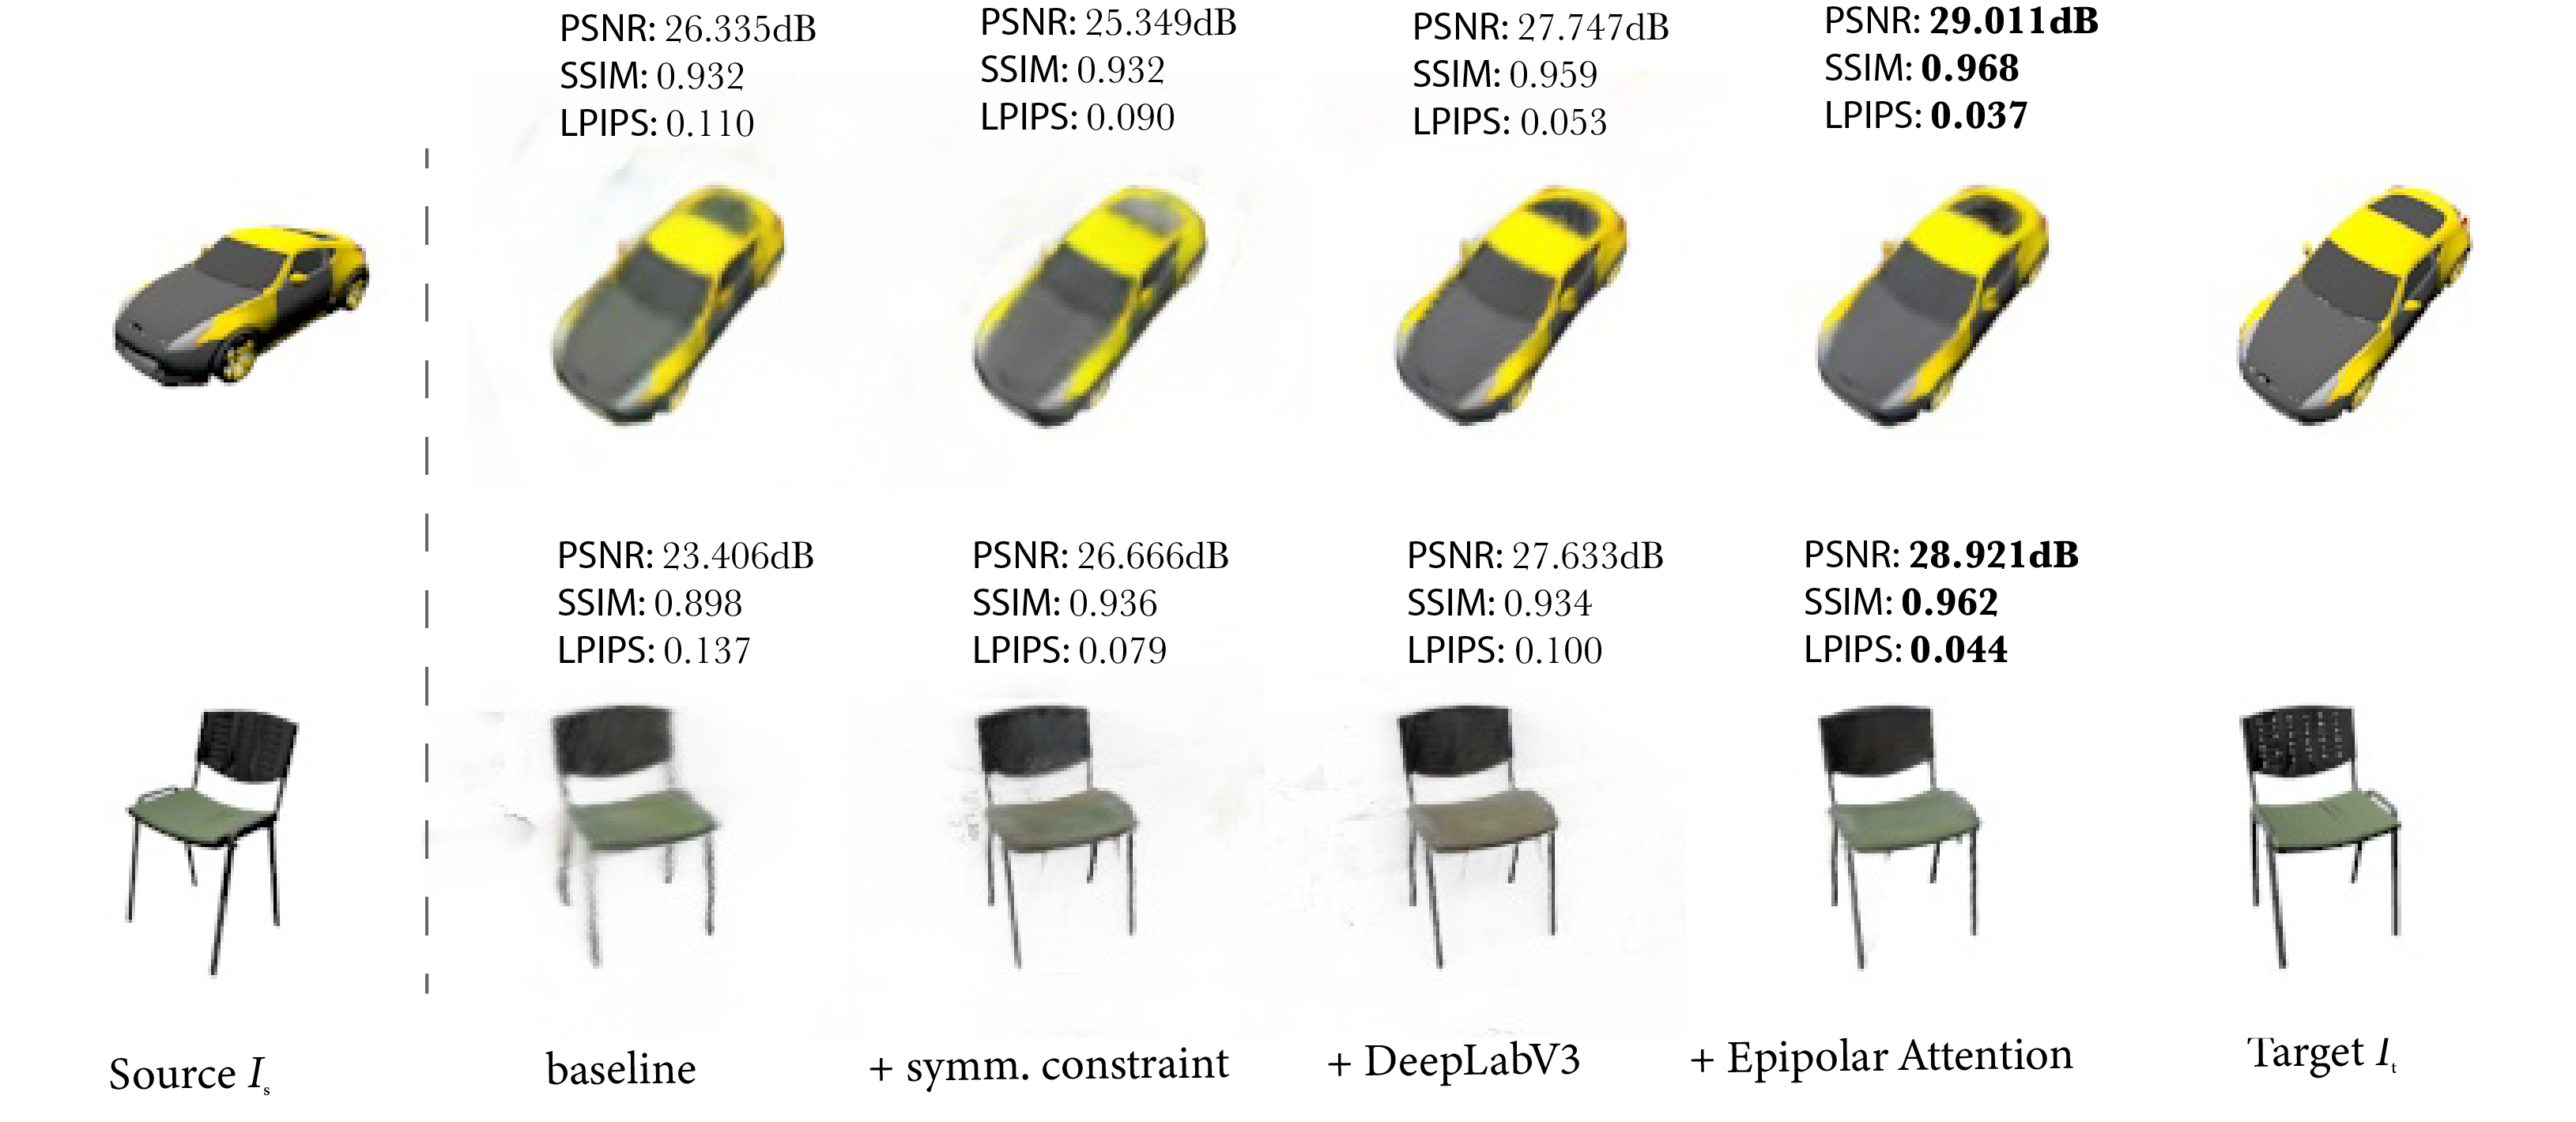
\includegraphics[width=\linewidth]{images/epinerf/supp_ablation_illustration.png}
  \caption{\textbf{Ablation study.} Visual influence of the different modules and constraints that were progressively applied to our architecture on ShapeNet-SRN dataset.}
  \label{fig:ablation}
  \end{center}
\end{figure}  


\subsection{Additional results - Standford Cars dataset }
We finally evaluate our EpiNeRF architecture using real-world images from the Stanford Cars dataset  \citep{krause20133d}. First, raw images were segmented with the state-of-the-art segmentation model SAM \citep{kirillov2023segment}. These background-free images were then scaled and centered to match the ShapeNet-SRN image structure. Although such a testing scenario is far from the one our architecture has been trained for, Figure \ref{fig:res_Stanfordcar} demonstrates that EpiNeRF produces sharper results compared to SymmNeRF \citep{li2022symmnerf}, even though reliable camera pose information is missing.


\begin{figure}[h!]
    \begin{center}
  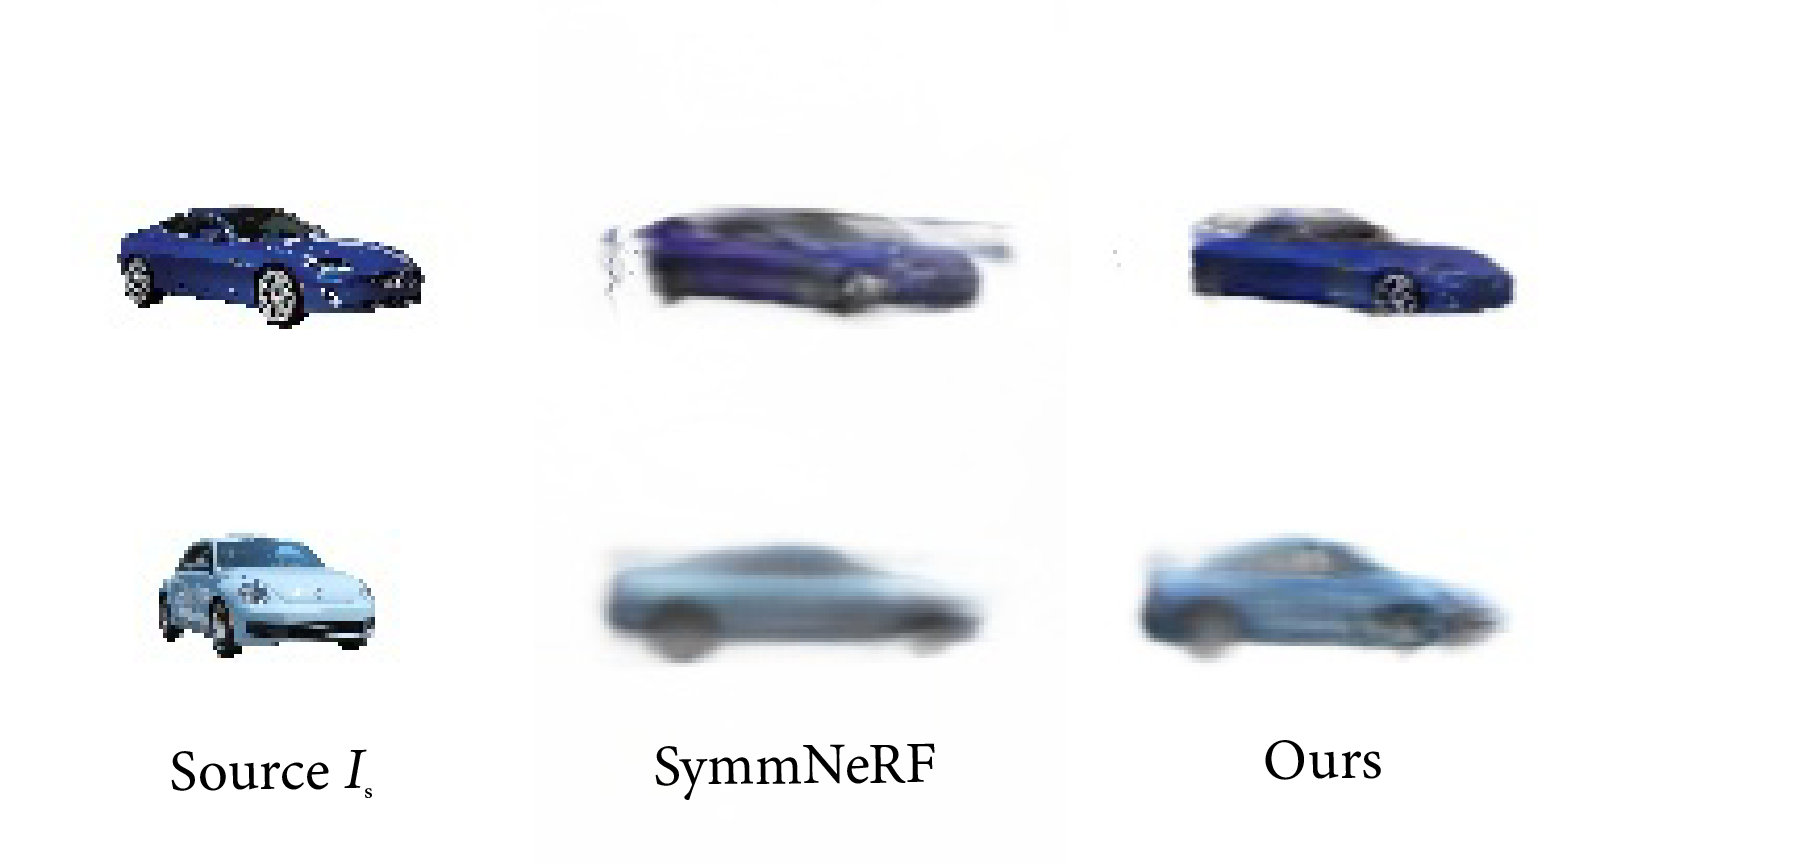
\includegraphics[width=\linewidth]{images/epinerf/supp_CarsStandford.png}
  \caption{\textbf{Novel view synthesis on Stanford \textit{Cars} dataset} \citep{krause20133d}. Whereas even closed target viewpoint from the source view leads to fuzzy results, our method render sharper results than SymmNeRF \citep{li2022symmnerf}. }
  \label{fig:res_Stanfordcar}
  \end{center}
\end{figure}

\subsection{Feature and attention: visual insights}
\label{subsec:visual_insights}

\noindent \textbf{Feature generation from CNN $\chi$ and NeRFeature $\Psi$.} The Figure \ref{fig:feature_illustration} presents few first-channel feature volumes obtained from different \textit{Cars} and \textit{Chairs} instances by $\chi$. Our image features has a 128$\times$128 spatial resolution whereas SymmNeRF produces a low  64$\times$64 resolution feature volume. 

\begin{figure}[h!]
\begin{center}
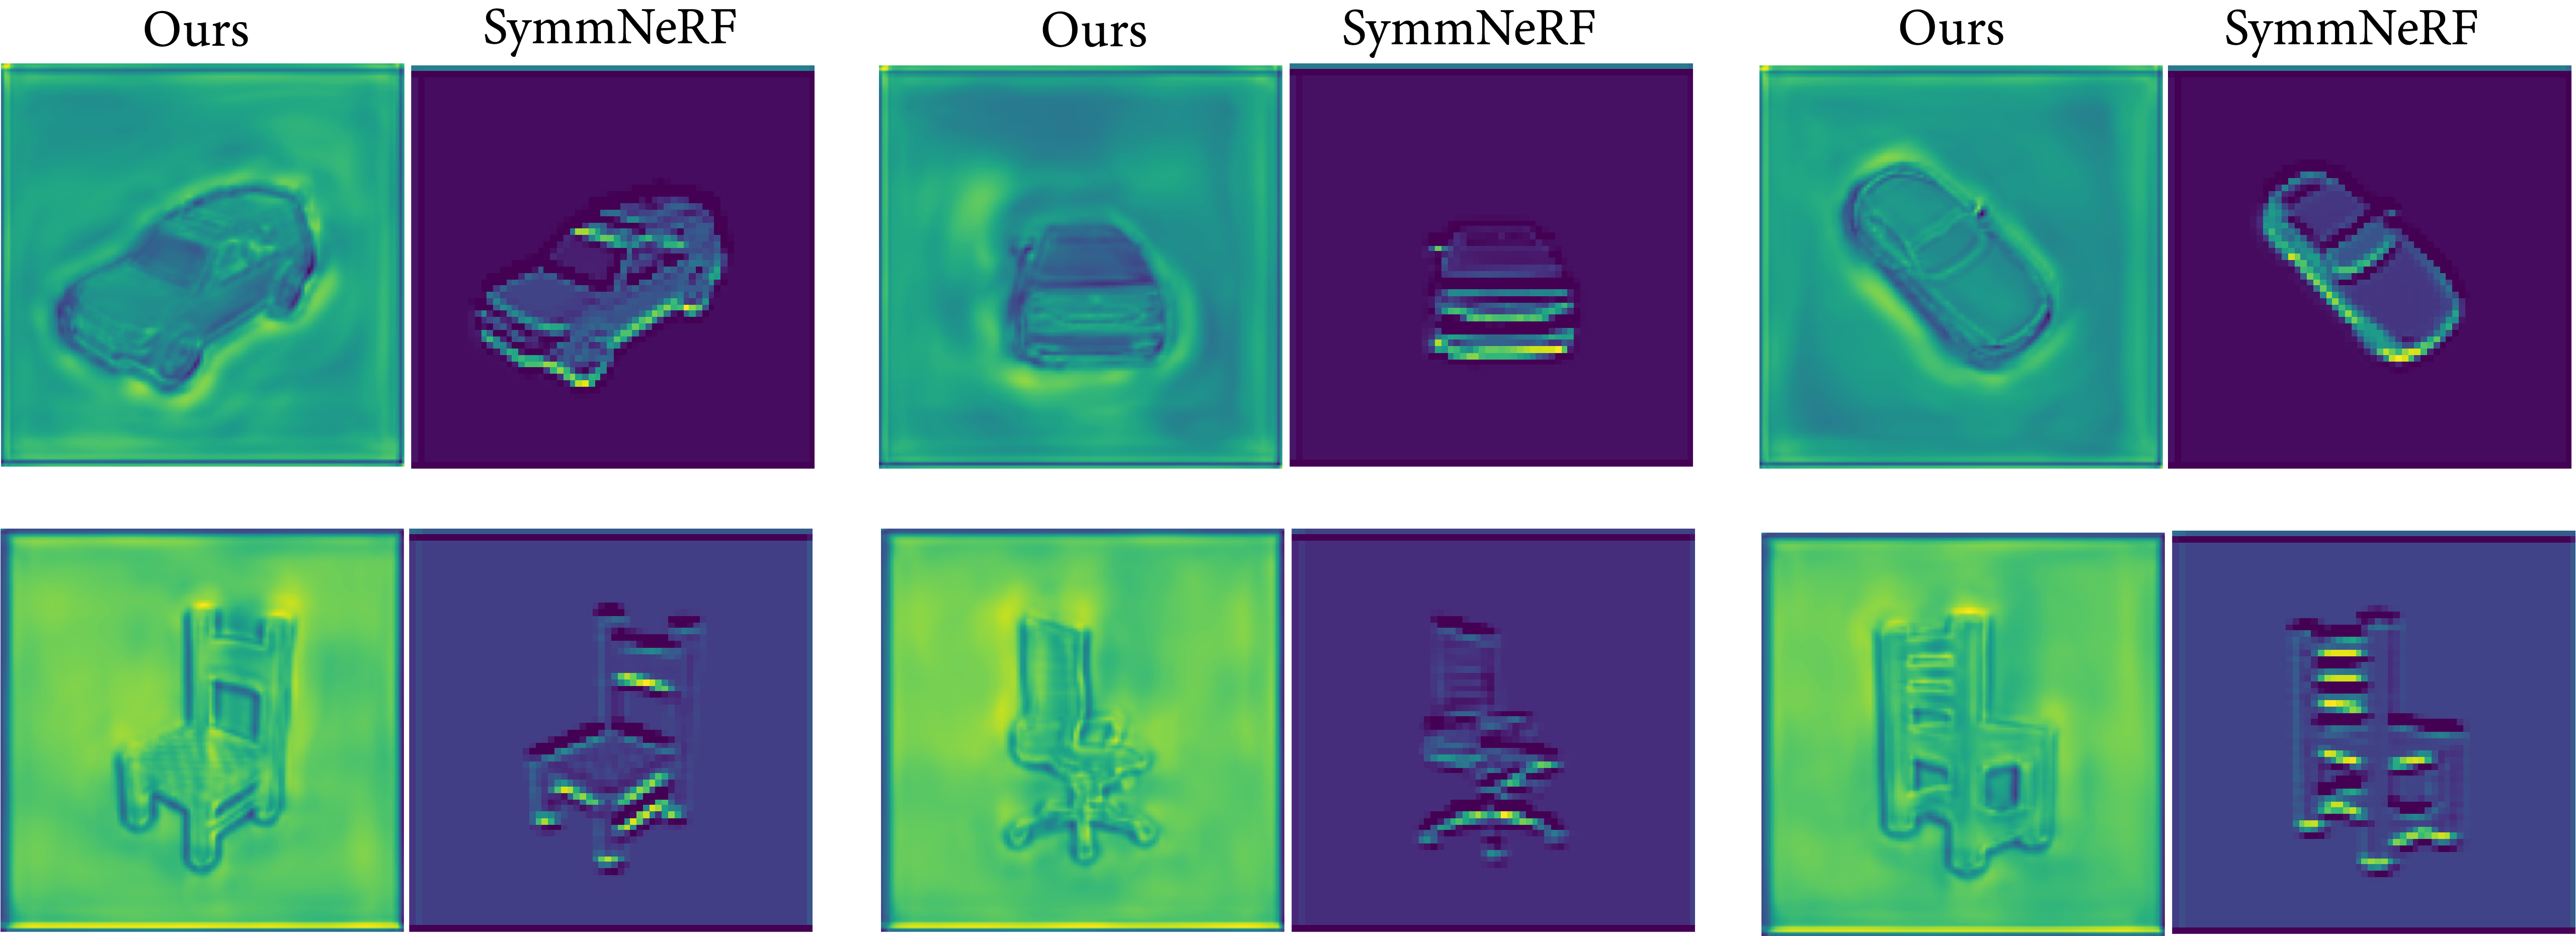
\includegraphics[width=\linewidth]{images/epinerf/feature_supp_NEW.png}
   \caption{\textbf{Feature map produced by our encoder $\chi$ and by SymmNeRF.} Features produced by $\chi$ contain detailed patterns that SymmNeRF struggles to handle at half the resolution of the input image size.}
\label{fig:feature_illustration}
\end{center}
\end{figure} 

Higher resolution feature volumes allow for more accurate pixel-wise local sampling. In contrast, using a low-resolution feature volume, such as the one employed in SymmNeRF, results in coarser pixel sampling.

The primary purpose of NeRFeature is not to generate a complete feature volume from a target viewpoint. EpiNeRF requires only pixel-wise target-aligned features to compute the epipolar cross-attention feature distribution $\mathbf{s}_{a}$. A complete deep feature volume $\mathbf{F}_{t}$ is shown in Figure \ref{fig:feat_and_att} (a) for an illustrative purpose. Our feature radiance field $\Psi$ thus accurately infers the overall position of the target car, although it may not capture fine details (\eg windows) with complete accuracy. The feature volumes produced by $\chi$ in the target view $I_{t}$ are used as pseudo-ground truth to supervise the training of NeRFeature $\Psi$. \newline

\begin{figure}[htp!]
  \centering
  \begin{subfigure}{0.48\linewidth}
    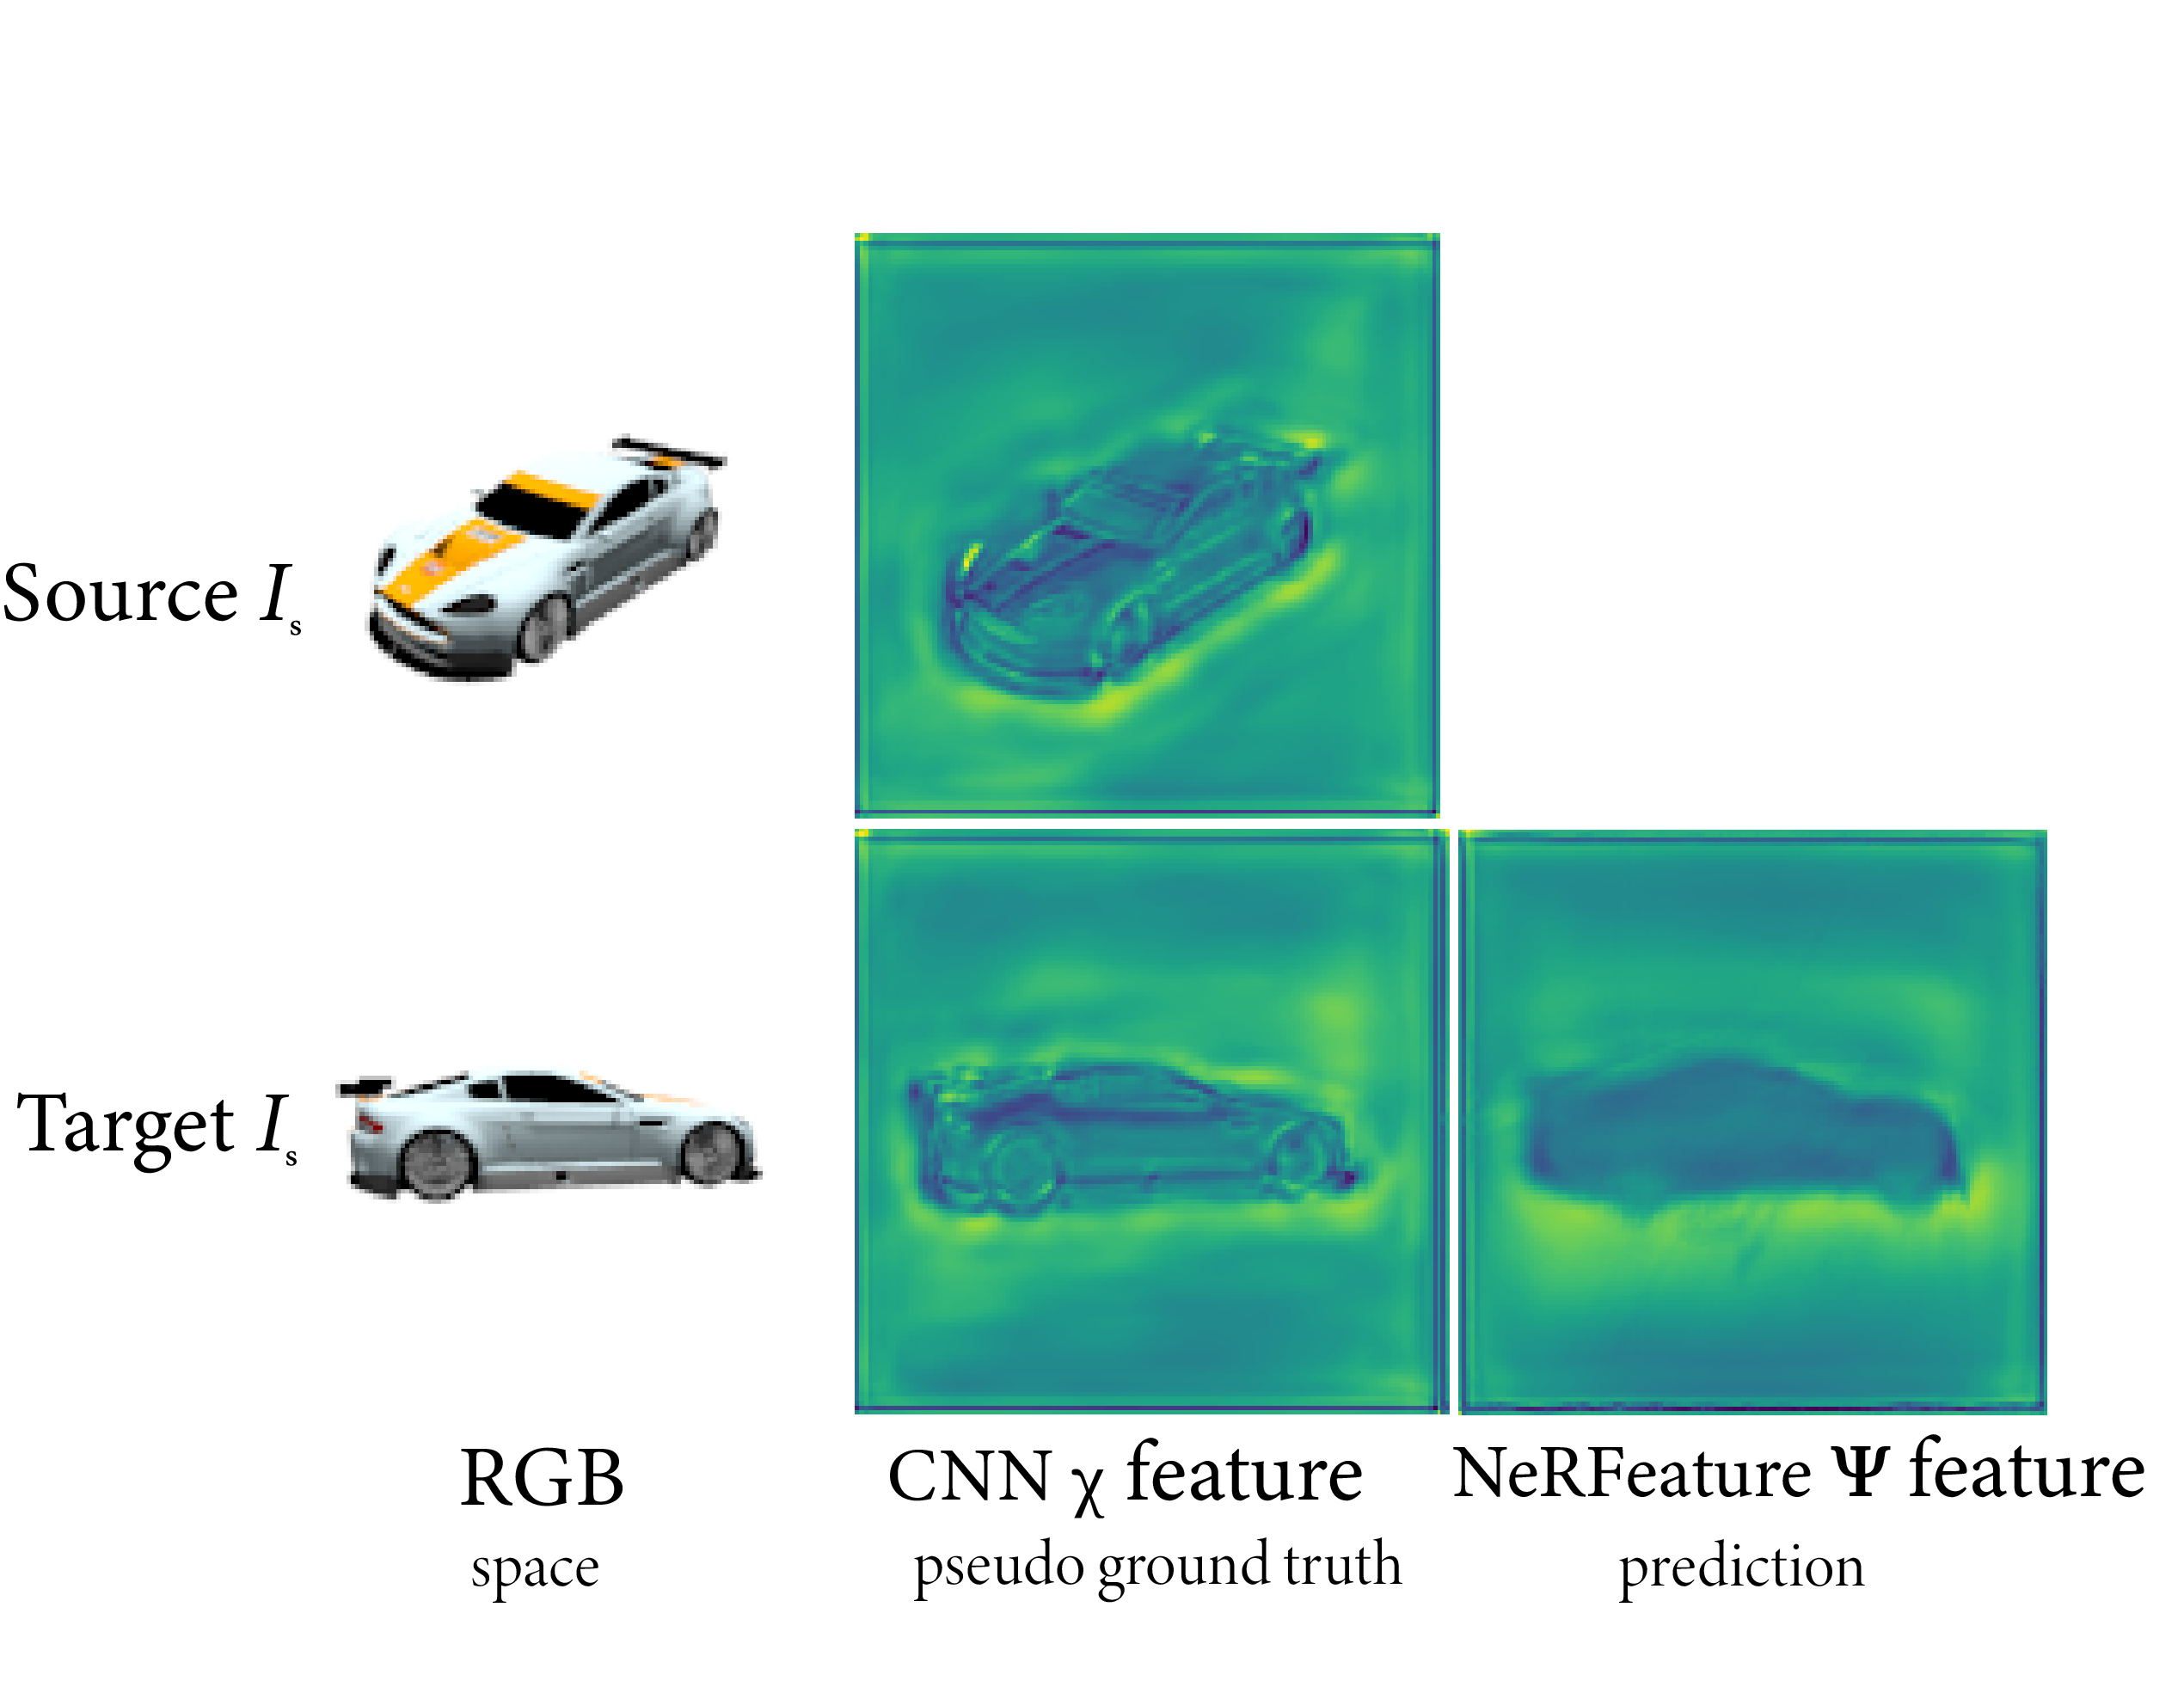
\includegraphics[width=\linewidth]{images/epinerf/nerfeature-main.png}
    \caption{}
    \label{fig:short-a}
  \end{subfigure}
  \hfill
  \begin{subfigure}{0.48\linewidth}
    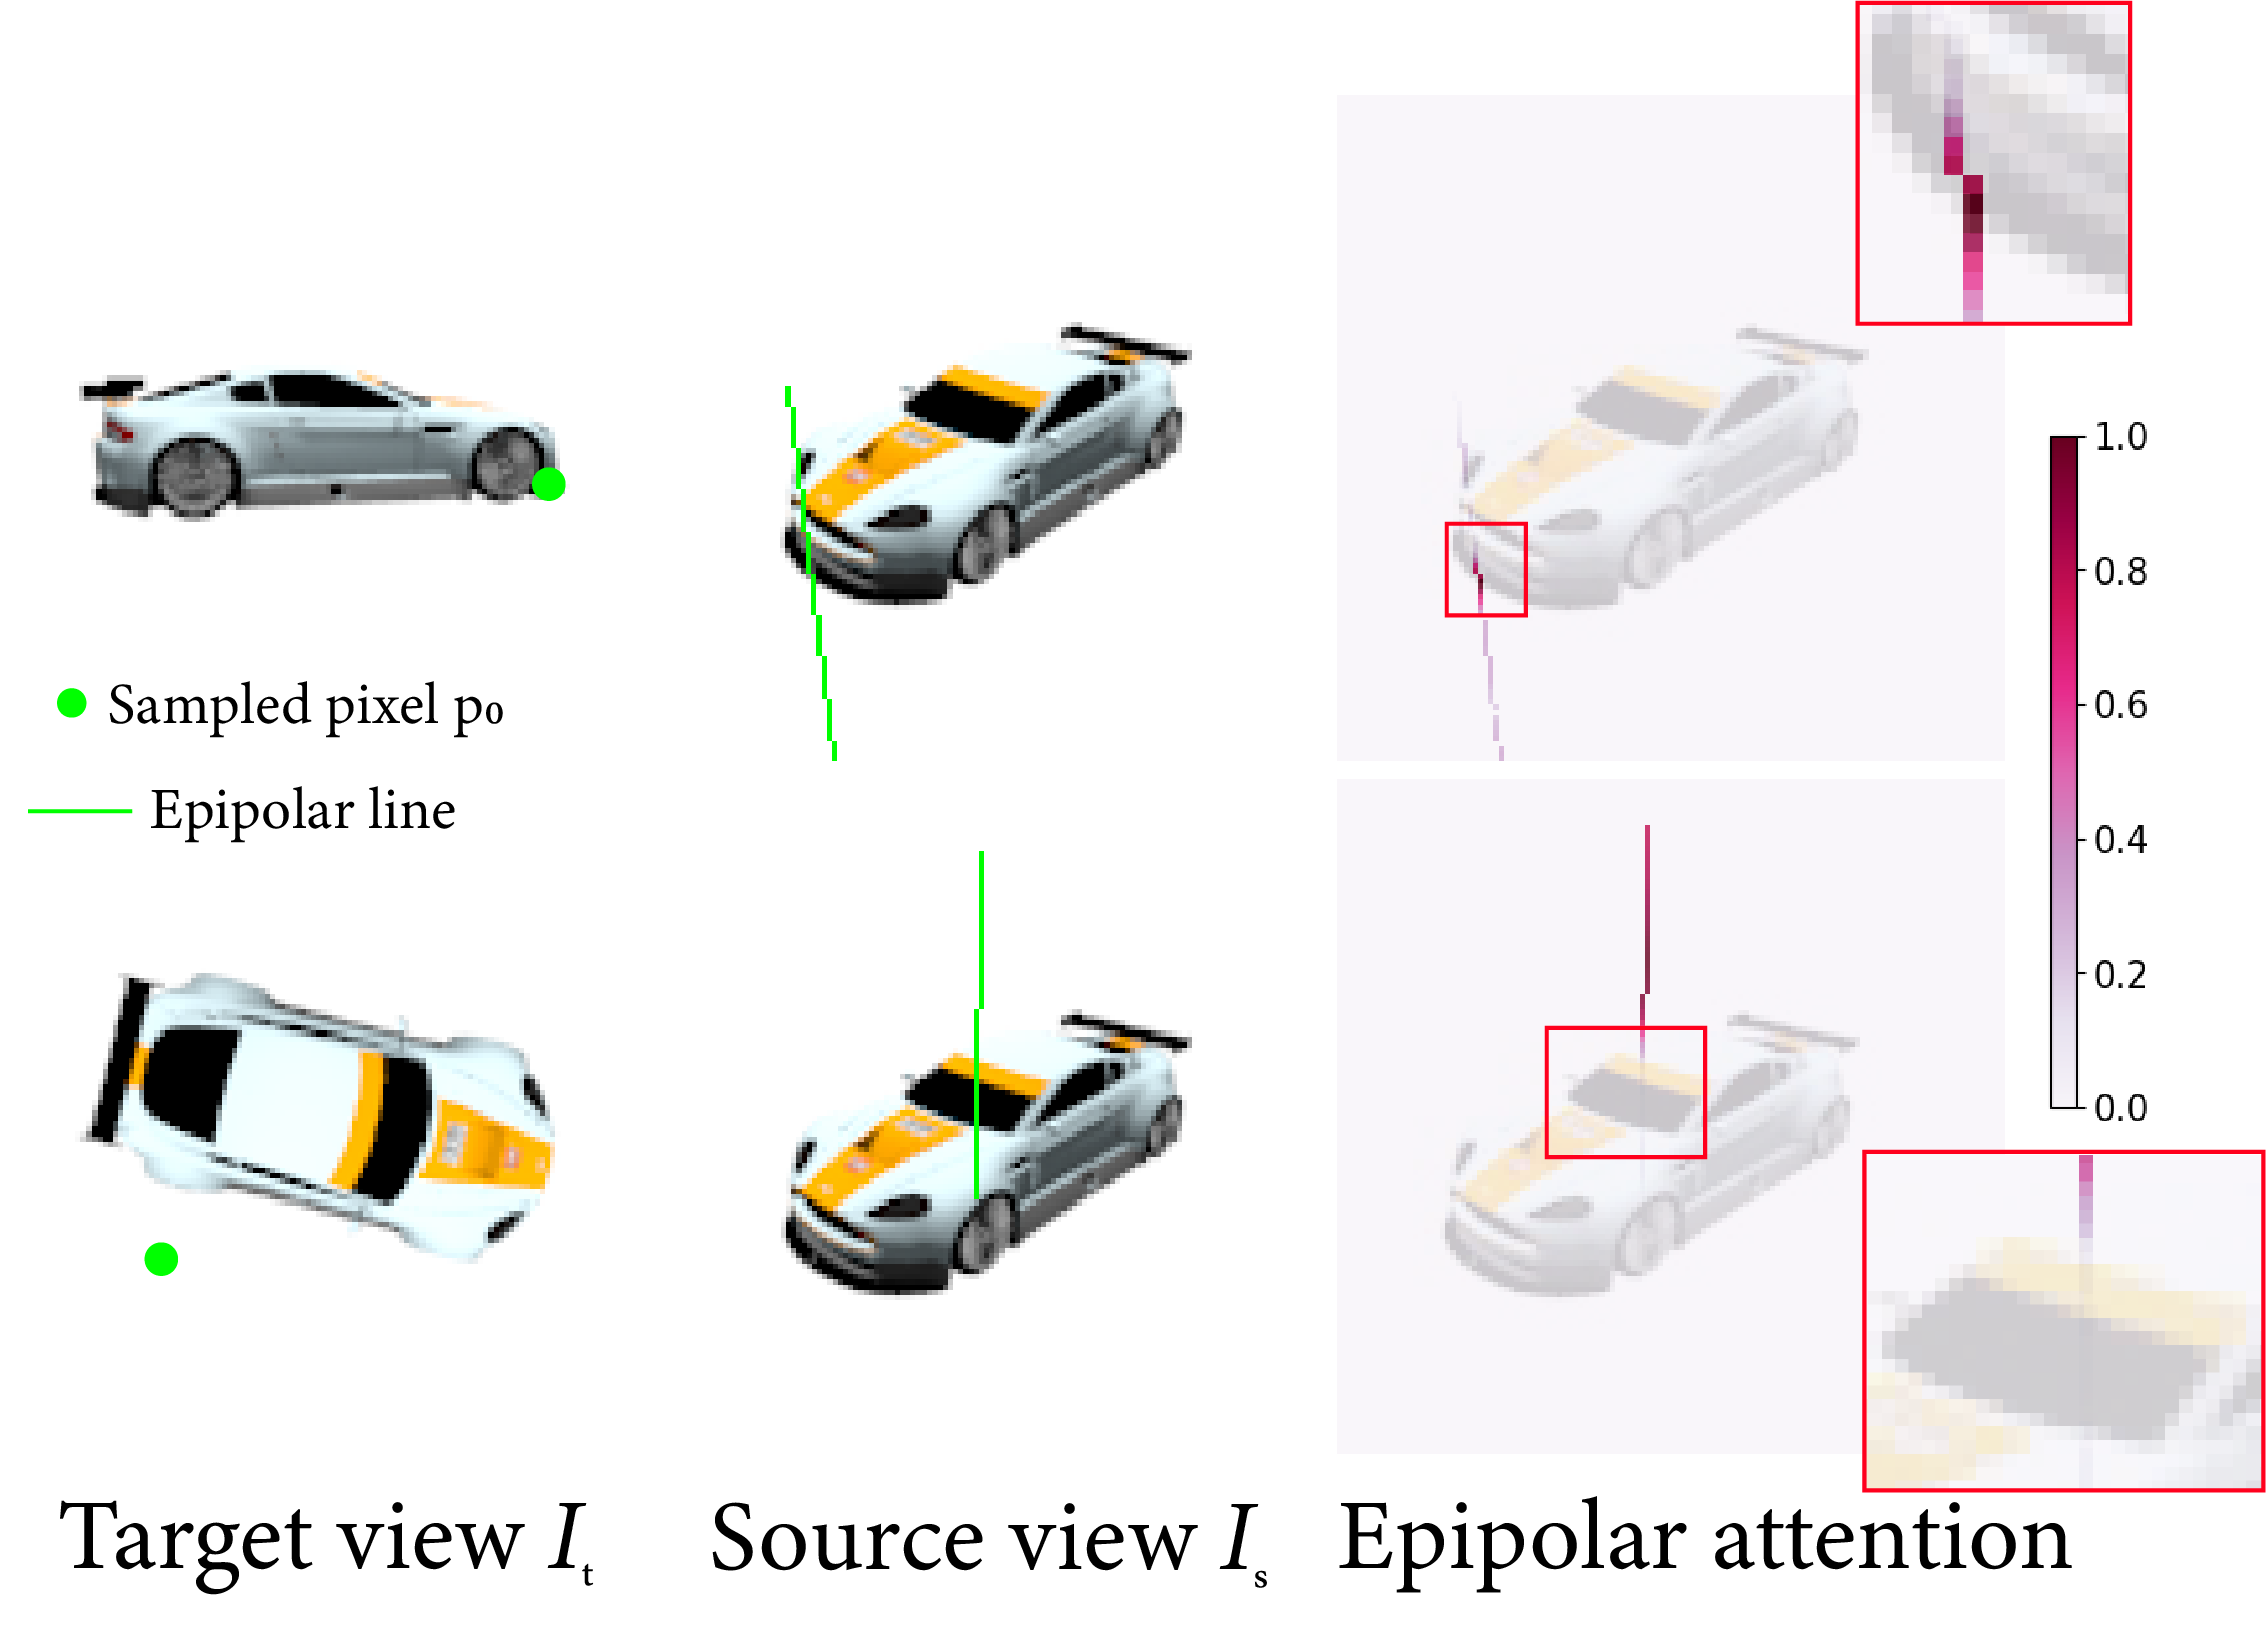
\includegraphics[width=\linewidth]{images/epinerf/attention_main.png}
    \caption{}
    \label{fig:short-b}
  \end{subfigure}
  \caption{\textbf{Visual insights regarding NeRFeature and our epipolar attention mechanism.} (a) \textit{Pseudo} ground truth features are generated through our CNN encoder-decoder $\chi$. (b) Epipolar attention activation in two different scenarios.}
\label{fig:feat_and_att}
\end{figure}

\noindent \textbf{Epipolar attention.}
Figure \ref{fig:feat_and_att} (b) depicts visuals insights into our epipolar attention module. For a pixel $p_{0}$ sampled on the target view, the corresponding epipolar line is drawn in the source domain as a green line. As illustrated on the first row, if $p_{0}$ is sampled from the front right wheel, the attention distribution along the epipolar line shows its highest activation near the same region. It occurs even though the wheel is no longer visible in the source view. Conversely, when $p_{0}$ is sampled from an empty background area (bottom row), higher attention scores are observed along the epipolar line until it crosses the car roof. 

We finally illustrate in Figure \ref{fig:attention_overview} an example to demonstrate how our epipolar attention mechanism influences the final weight distribution and, consequently, the rendered color. The middle row presents both the raw and normalized attention distributions, along with our final attention-based weight distribution.   The last two rows show that our feature cross-attention distribution aims to focus on \textit{source-view} regions that semantically match the pixel sampled from the target viewpoint (\eg on the bottom part of the door rather than on the window) even if this region is unobserved in the source viewpoint. 

\begin{figure}[htp!]
    \begin{center}
  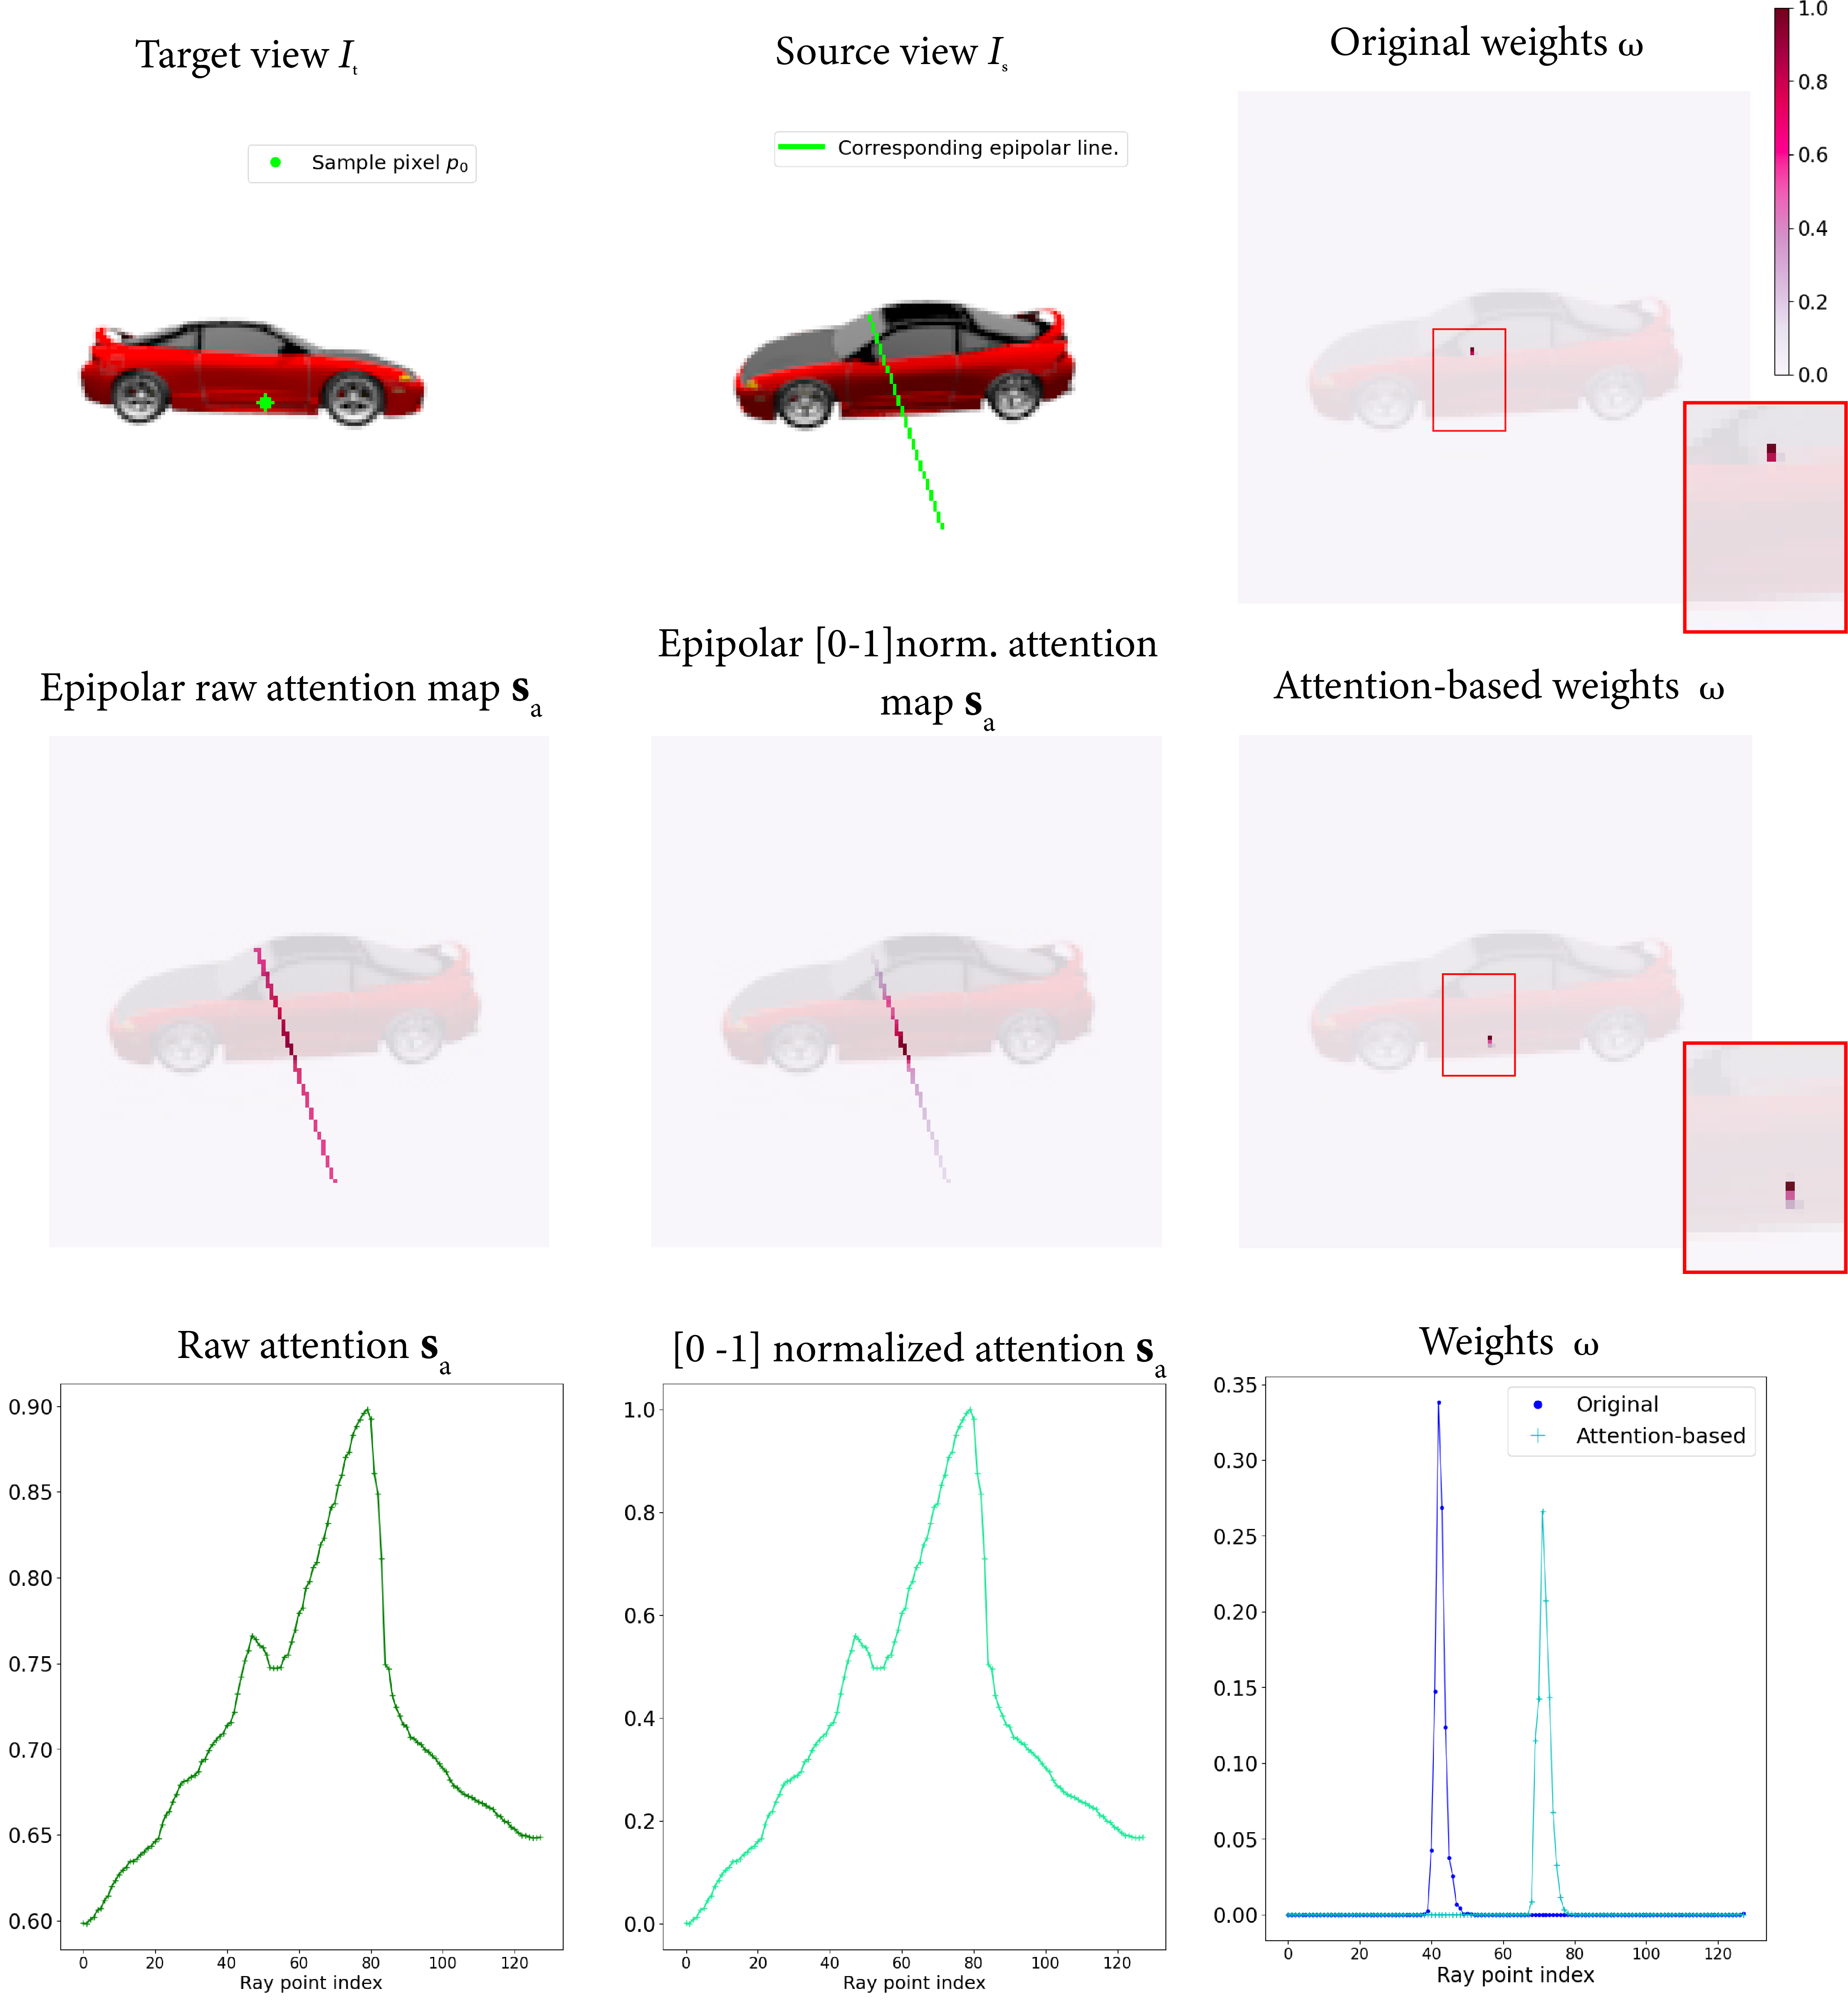
\includegraphics[width=\linewidth]{images/epinerf/SUPP_COMPLETE_OVERVIEW_OVERLEAF.png}
  \caption{\textbf{Illustration of our feature-based attention mechanism.} Sampled pixel $p_{0}$ on the target view $I_{t}$ and the associated epipolar line on the source view $I_{s}$ are presented in the first row, with the original weight distribution. }
  \label{fig:attention_overview}
  \end{center}
\end{figure}

Our epipolar attention-based volume rendering correction emphasises the need for the ray to terminate later ($\sim$ \textit{index} $80^{th}$), as opposed to the initial prediction ($\sim$ \textit{index} $50^{th}$). Additional information is available in the supplementary material.

\section{Conclusion}

We introduced in this chapter EpiNeRF, a novel \ac{NeRF}-based architecture for single-image \ac{NVS}. The key innovation of EpiNeRF lies in the integration of an epipolar constraint into the RGB volume rendering process. This constraint is implemented using a lightweight feature-based attention mechanism, allowing EpiNeRF to improve the sampling of 3D points. As a result, it visually produces more appealing novel views compared to current state-of-the-art methods.

Our method can be summarised as follows: Source-aligned features that are produced by a pre-trained 2D CNN encoder $\chi$ are distilled into a 3D feature radiance field, termed NeRFeature. This generalizable radiance field, conditioned on the source-aligned features, is designed to produce target-aligned features. This prior information, which helps for addressing occlusions, is typically unavailable in single-image \ac{NVS} methods. Finally, both source and target-aligned features are used in a lightweight, epipolar attention-based module during the fine-tuning of our EpiNeRF architecture. We demonstrated through extensive experiments and ablation studies the significant impact our feature-based epipolar constraint has on novel view synthesis.

EpiNeRF seeks to improve the integration of 3D priors into neural radiance fields by incorporating a feature-based epipolar constraint within generalizable NeRF architectures for single-image \ac{NVS}.
